\documentclass[10pt]{beamer}
\usetheme[
%%% options passed to the outer theme
    hidetitle,           % hide the (short) title in the sidebar
    hideauthor,          % hide the (short) author in the sidebar
%    hideinstitute,       % hide the (short) institute in the bottom of the sidebar
%    shownavsym,          % show the navigation symbols
%    width=2cm,           % width of the sidebar (default is 2 cm)
%    hideothersubsections,% hide all subsections but the subsections in the current section
%    hideallsubsections,  % hide all subsections
%    left                % right of left position of sidebar (default is right)
  ]{Aalborg}
  
% If you want to change the colors of the various elements in the theme, edit and uncomment the following lines
% Change the bar and sidebar colors:
%\setbeamercolor{Aalborg}{fg=red!20,bg=red}
%\setbeamercolor{sidebar}{bg=red!20}
% Change the color of the structural elements:
%\setbeamercolor{structure}{fg=red}
% Change the frame title text color:
%\setbeamercolor{frametitle}{fg=blue}
% Change the normal text color background:
%\setbeamercolor{normal text}{bg=gray!10}
% ... and you can of course change a lot more - see the beamer user manual.

\usepackage[utf8]{inputenc}
\usepackage[english]{babel}
\usepackage{geometry}
\usepackage{array}
\usepackage{hhline}
\usepackage{hyperref}
\usepackage{pdfpages}
\usepackage{rotating}
\usepackage[T1]{fontenc}
% Or whatever. Note that the encoding and the font should match. If T1
% does not look nice, try deleting the line with the fontenc.
\usepackage{helvet}
\usepackage{tabularx}	
\usepackage{multirow}                   % Tabelfunktion
\usepackage{multicol}                   % Tabelfunktion
\usepackage{wrapfig}	
\usepackage{import}					%For at importere svg med latex font
\usepackage{longtable}
\usepackage{color} 
\usepackage{colortbl}
\usepackage{graphicx}
\usepackage[compatibility=false]{caption}
\usepackage{subcaption}
\usepackage{epstopdf}






\definecolor{textBlue}{rgb}{0.90, 0.94, 1}    % {0.95, 0.98, 1}

% colored hyperlinks
\newcommand{\chref}[2]{%
	\href{#1}{{\usebeamercolor[bg]{Aalborg}#2}}%
}

% specify the logo in the top right/left of the slide
\pgfdeclareimage[height=1cm]{mainlogo}{images/AAUgraphics/aau_logo_new} % placed in the upper left/right corner
\logo{\pgfuseimage{mainlogo}}

\graphicspath{{images/}}



\begin{document}
% the titlepage
\newgeometry{top=-96mm, bottom=0cm, outer=0cm, inner=0cm, marginparwidth=0cm, marginparsep=0cm}

\includepdf{thesis_presentation.pdf}
\restoregeometry

%{\aauwavesbg
%\begin{frame}[plain,noframenumbering] % the plain option removes the sidebar and header from the title page
%  \titlepage
%\end{frame}}

\section{Agenda}
\begin{frame}{Agenda}{}
%\tableofcontents
\begin{block}{De næste ca. 30 min.:}
  \begin{itemize}
    \item Baggrund og metoder til at løse problemet \textit{(Britt)}
    \item Design af en sikker regulator \textit{(Christian)}
    \item Analyse af en arbitrær regulator \textit{(Britt)}
    \item Konklusion \textit{(Christian)}
  \end{itemize}
\end{block}
\begin{block}{Derudover:}
  \begin{itemize}
    \item Demo i lab som tiden tillader det
    \item Diskussion og spørgsmål
  \end{itemize}
\end{block}
\vspace{1cm}
\end{frame}
\section{Kirurgirobotik}
\begin{frame}{da Vinci på AAU}{Robotteknologi indenfor kirurgi}
%\tableofcontents
%\begin{minipage}[b]{0.55\linewidth}
\vspace{8mm}
\begin{block}{Incitament for projektet}
	\begin{itemize}
		\item \href{file:video/surgery_robotics_history_davinci_chart.mp4}{Udbredelse og udvikling indenfor kirurgirobotik}
		\item AAU: Patient-manipulator afkoblet fra master-konsol 
		\item \href{file:video/davinci_joints.mp4}{Kontrollerbare robotled}
		\item Sikkerhed ved robotoperationer
		\item Fremtiden for robotkirurgi
		\item Mål med projektet
		\item Implementation i ROS
		\item To tilgangsvinkler
	\end{itemize}
\end{block}
%\vspace{3mm}
%\begin{block}{Semi-automatisering}
%	\begin{itemize}
%		\item Virtuelle fiksturer -- mindske risiko ved operation
%		\item Garanti for patientsikkerhed
%	\end{itemize}
%\end{block}
%\end{minipage}
%	\hspace{0.1cm}
%\begin{minipage}[b]{0.42\linewidth}
\begin{flushright}
	\vspace{-30mm}

\includegraphics[width=0.5\textwidth]{coffee_robot.png}
\end{flushright}
%\end{minipage}
\vspace{1cm}
\end{frame}

%\section{Kirurgirobot på AAU}
%\begin{frame}{Kirurgirobotten på Aalborg Universitet}{Første-generations da Vinci-robot}
%\begin{minipage}[b]{0.55\linewidth}
%	\vspace{2mm}
%\begin{block}{Modificeret da Vinci-robot}
%	\begin{itemize}
%		\item
%	\end{itemize}
%\end{block}
%\vspace{-1mm}
%\begin{block}{Fokus på sikkerhed}
%	\begin{itemize}
%		\item Barrierecertifikater til garanti af sikkerhed
%		\item Design af sikkerhedsregulator vha. kontrolbarrierefunktioner
%		\item Sikkerhedsanalyse for lukketsløjfesystemer
%	\end{itemize}
%\end{block}
%\end{minipage}
%\hspace{0.1cm}
%%\vspace{-10mm}
%\begin{minipage}[b]{0.4\linewidth}
%	\begin{figure}[h]
%%		\vspace*{-5mm}
%		\centering
%		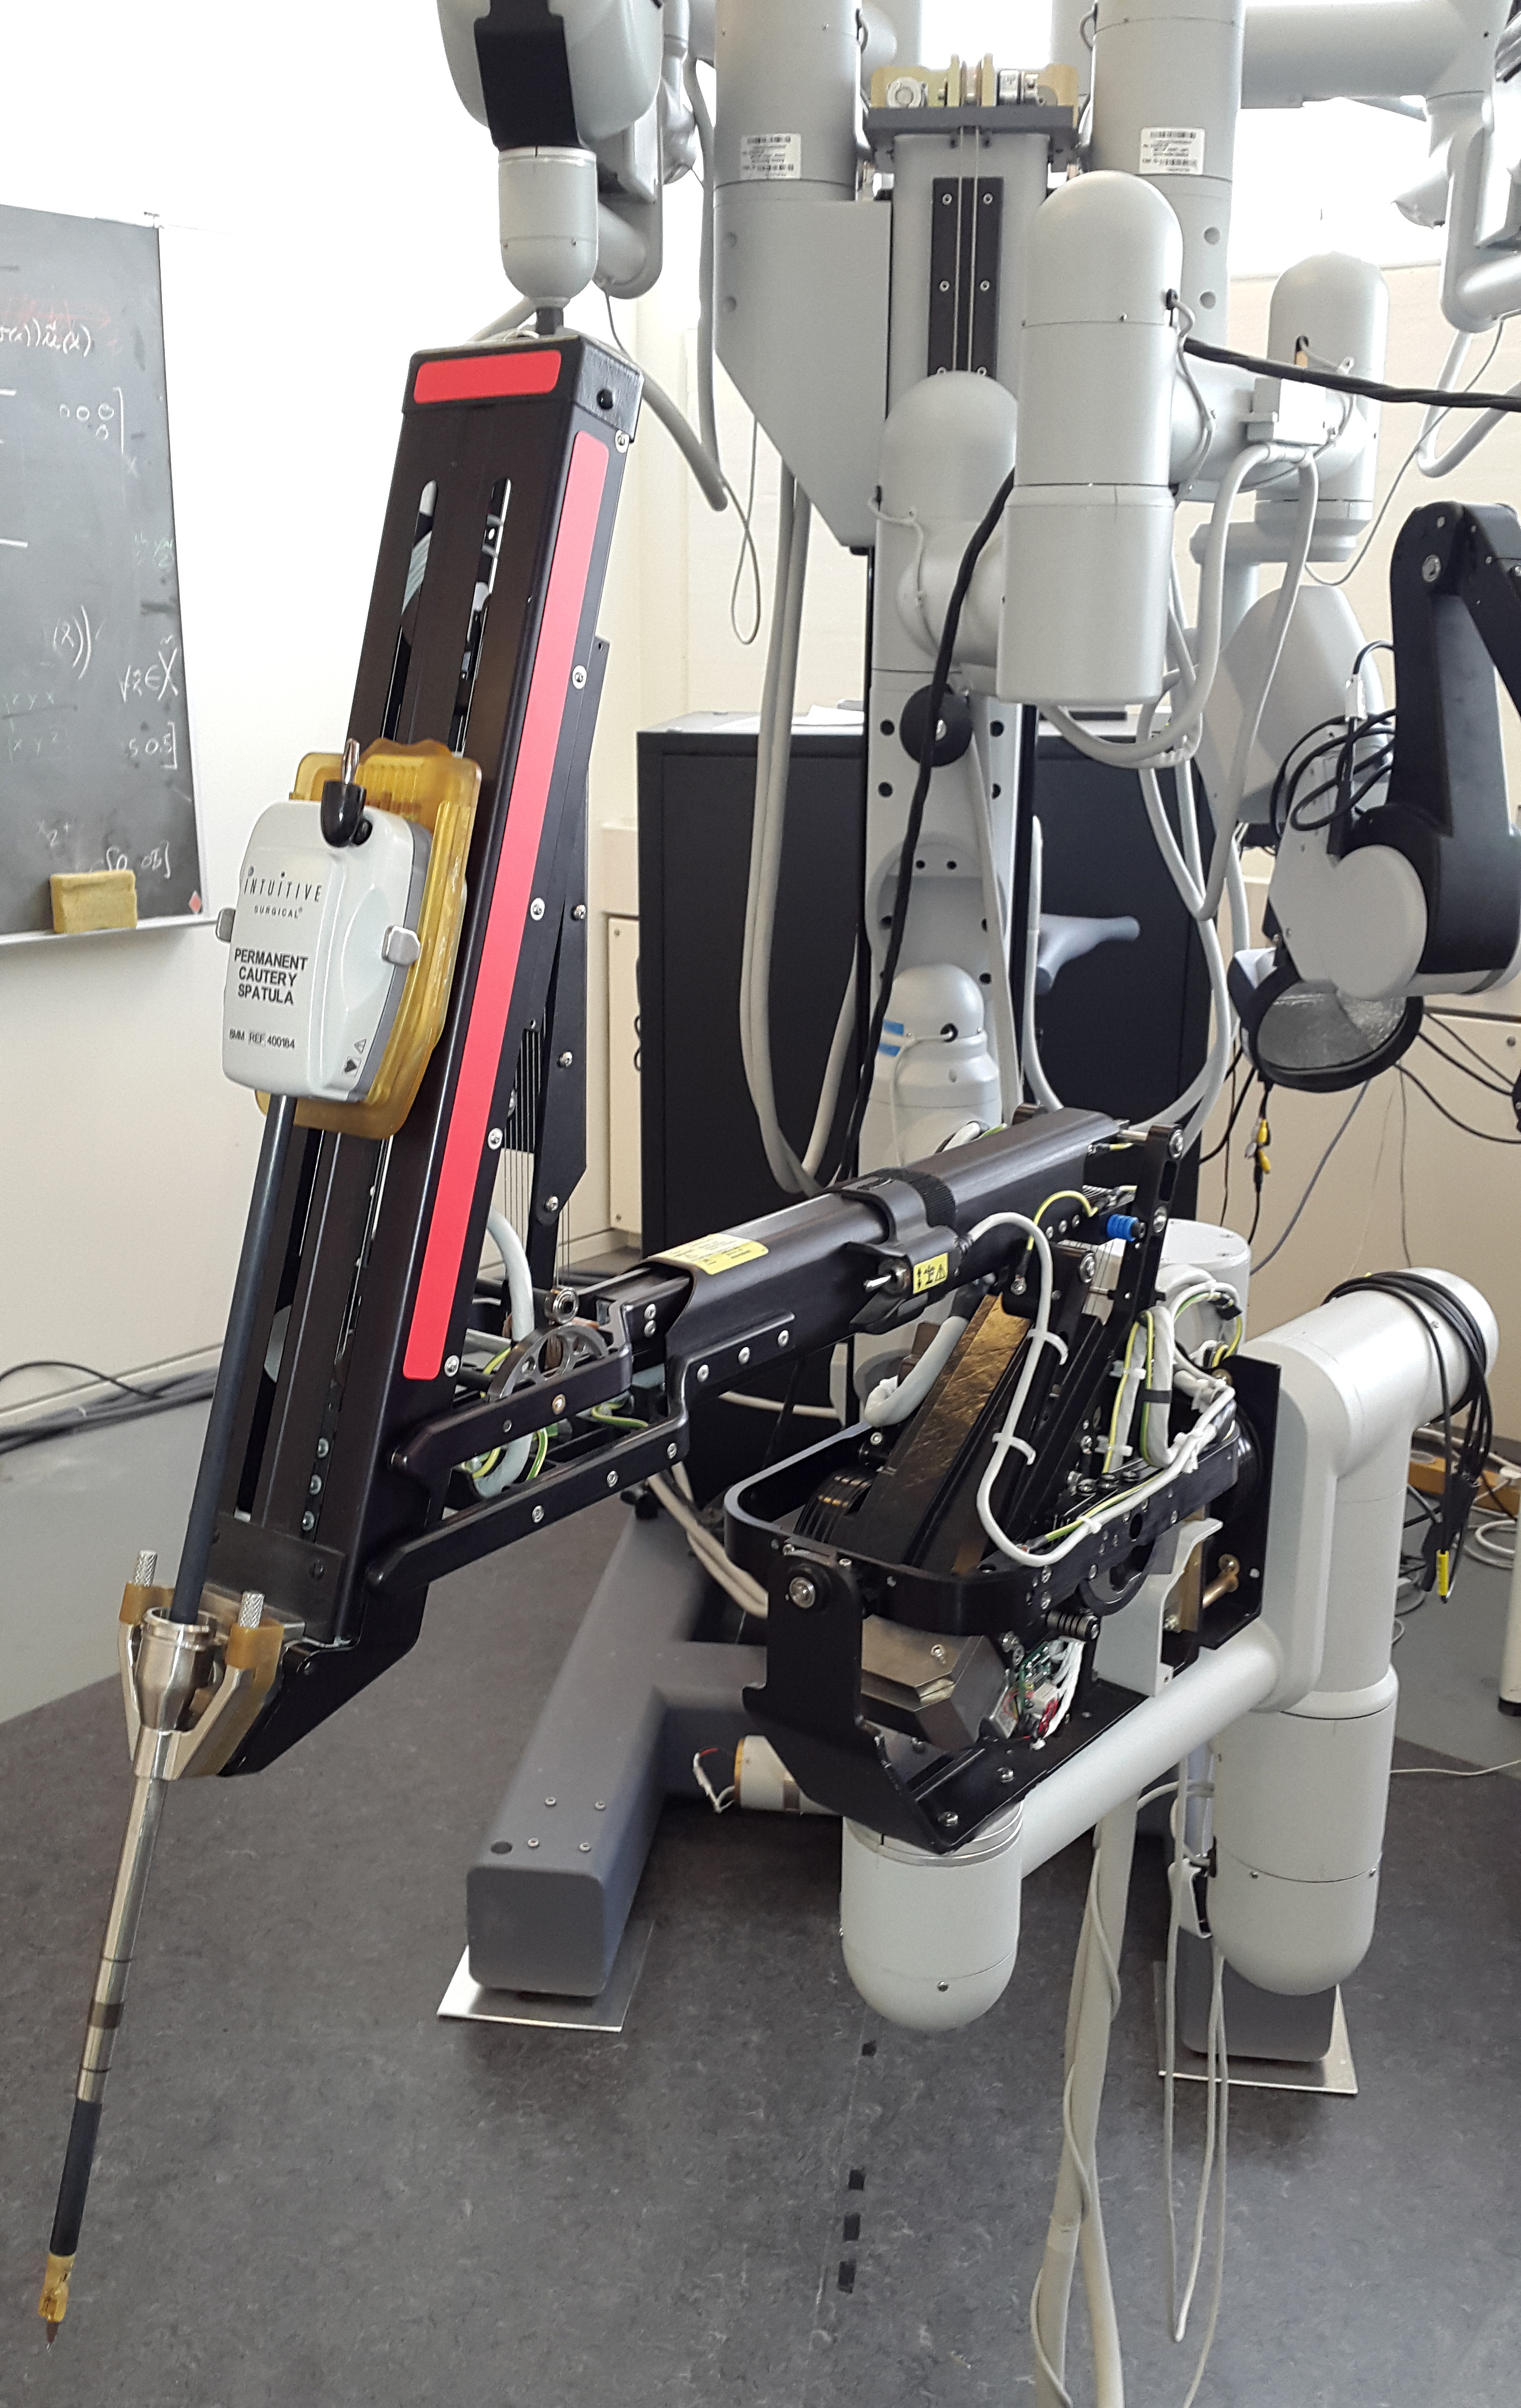
\includegraphics[width=1\textwidth]{20150517_120236.jpg}
%	\end{figure}
%\end{minipage}
%\vspace{1cm}
%\end{frame}

\section{Barrierecertifikater}
\begin{frame}{Barrierecertifikater}{Formelt bevis for garanteret sikkerhed}
\vspace{2mm}
\begin{block}{Definition af sikkerhed}
	\begin{itemize}
		\item Systemets tilstande er i $\mathcal{X}$
		\item Usikre tilstande er i $\mathcal{X}_u\subset\mathcal{X}$ og sikre tilstande i $\mathcal{X}_0\subseteq\mathcal{X}\setminus\mathcal{X}_u$
		\item Nulniveaukurven af $B(\textbf{x})$ danner  barriere mellem $\mathcal{X}_0$ og $\mathcal{X}_u$
	\end{itemize}
\end{block}
\begin{figure}[h]
	\centering
	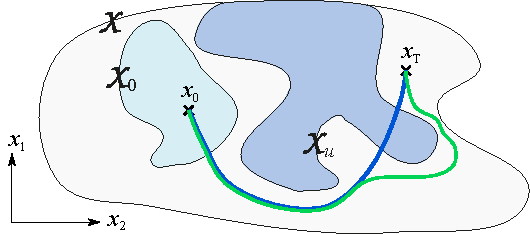
\includegraphics[width=0.8\textwidth]{safety.pdf}
\end{figure}
\vspace{1cm}
\end{frame}

\section{Kontroldesign}
\begin{frame}{Kontrolbarrierefunktioner (CBF)}{Konstruktion af CBF til design af sikkerhedsregulator}
	\vspace{2mm}
\begin{block}{To regulatorer}
	\begin{itemize}
		\item Lineær positionskontrol indenfor det sikre område $\mathcal{X}_0$
		\item Gradvis overgang til sikkerhedsregulator nær $\mathcal{X}_u$
		\item Designet vha. CLF så krav til sikkerhed bliver opfyldt
	\end{itemize}
\end{block}
\vspace{-2mm}
\begin{equation*}
u(\mathbf{x},\tilde{u})=\sigma(\mathbf{x})k_0(\mathbf{x})+(1-\sigma(\mathbf{x}))\tilde{u}(\mathbf{x})
\end{equation*}

\begin{figure}[h]
	\centering
	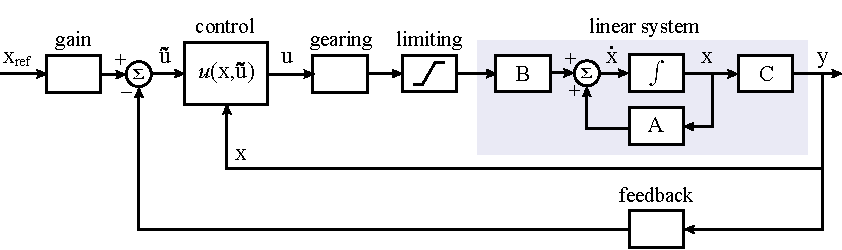
\includegraphics[width=0.9\textwidth]{control_system.pdf}
\end{figure}
	\vspace{5mm}
\end{frame}
\begin{frame}{Design fra CBF's}{Use-cases og fælles udfordringer}
\section{Design fra CBF's}
\begin{minipage}{0.5\textwidth}
	\begin{block}{Tre use-cases}
		\begin{itemize}
			\item Et "simpelt" case i 1D \\ \scriptsize{ - skabe erfaring med CBF's og den anvendte kontrol topologi}
			\item  \normalsize Virtual fixture \\ \scriptsize - at starte noget virkeligt anvendeligt
			\item \normalsize  Operationer i 3D rummet \\  \scriptsize - undgå at bringe vitale områder i fare
		\end{itemize}
	\end{block}
	\begin{block}{Fælles udfordringer\\ \scriptsize {\color{white}{lol}} - som vi møder som de første i Danmark}
		\begin{itemize}
			\item Konstruktion af CBF's \\ \scriptsize - som at lede efter Lyapunov funk.
			\item \normalsize Kontrol topologi
			\item Implementering på da Vinci med ROS
		\end{itemize}
	\end{block}
\end{minipage}
\hspace{0.3cm}
\begin{minipage}{0.45\textwidth}
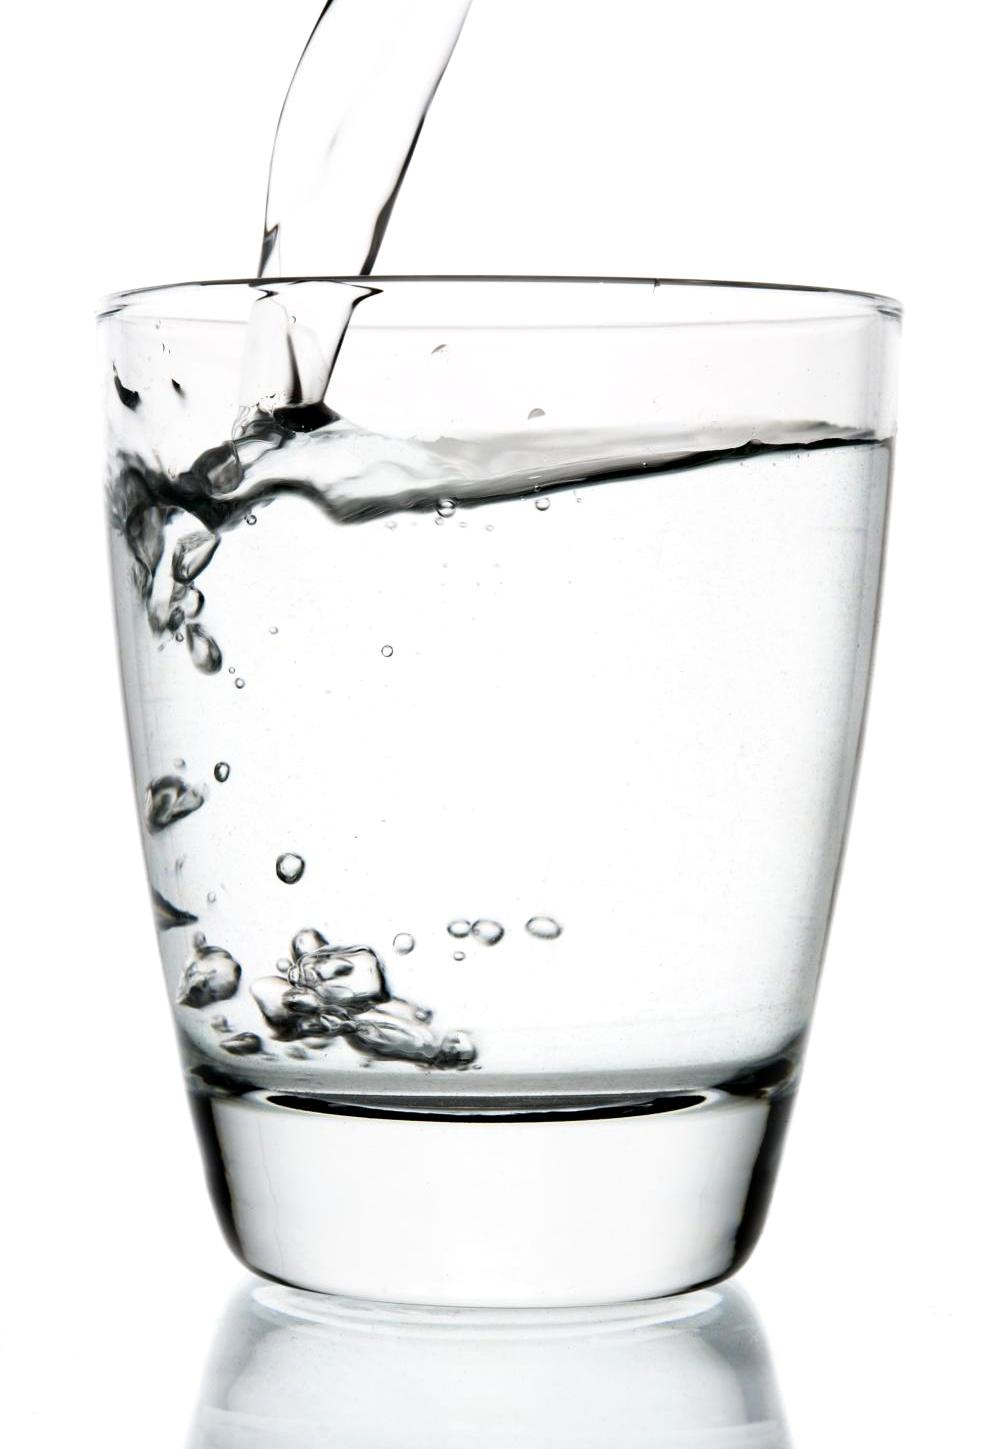
\includegraphics[width=0.35\linewidth]{simple}
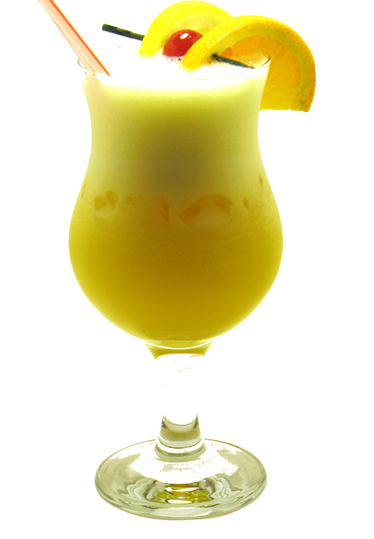
\includegraphics[width=0.35\linewidth]{tri.png}
\vspace{0.2cm}
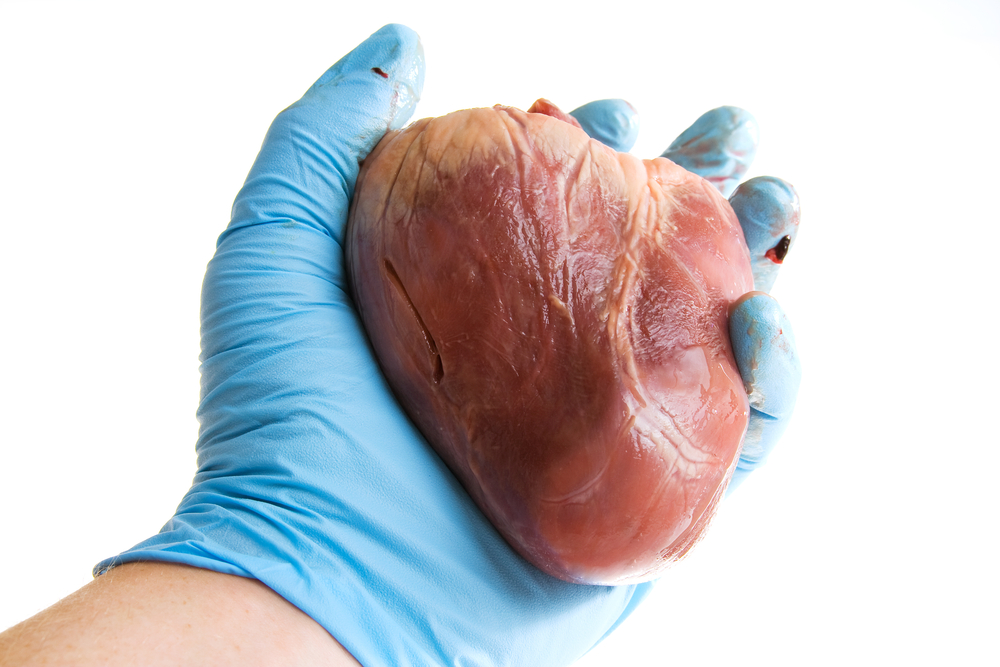
\includegraphics[width=0.6\linewidth]{human-heart.jpg}
\vspace{0.2cm}

\includegraphics[width=0.8\linewidth]{SIIB.jpg}
\vspace{0.2cm}
\end{minipage}
\end{frame}

\begin{frame}{Sikkerhed for et 1 dimensionelt system}{Det første skridt - instrument slide}
\section{Sikkerhed i 1D}
\vspace*{-0.5cm}
\begin{minipage}{0.6\textwidth}
\begin{block}{}
	\begin{itemize}
		\item Model
		\begin{itemize}
			\item 1. orden: Opnå erfaring
			\item 2. orden: Observer krævet
		\end{itemize}
		\item CBF
		\begin{itemize}
			\item parabel for 1. orden
			\item paraboloid for 2. orden
		\end{itemize}
			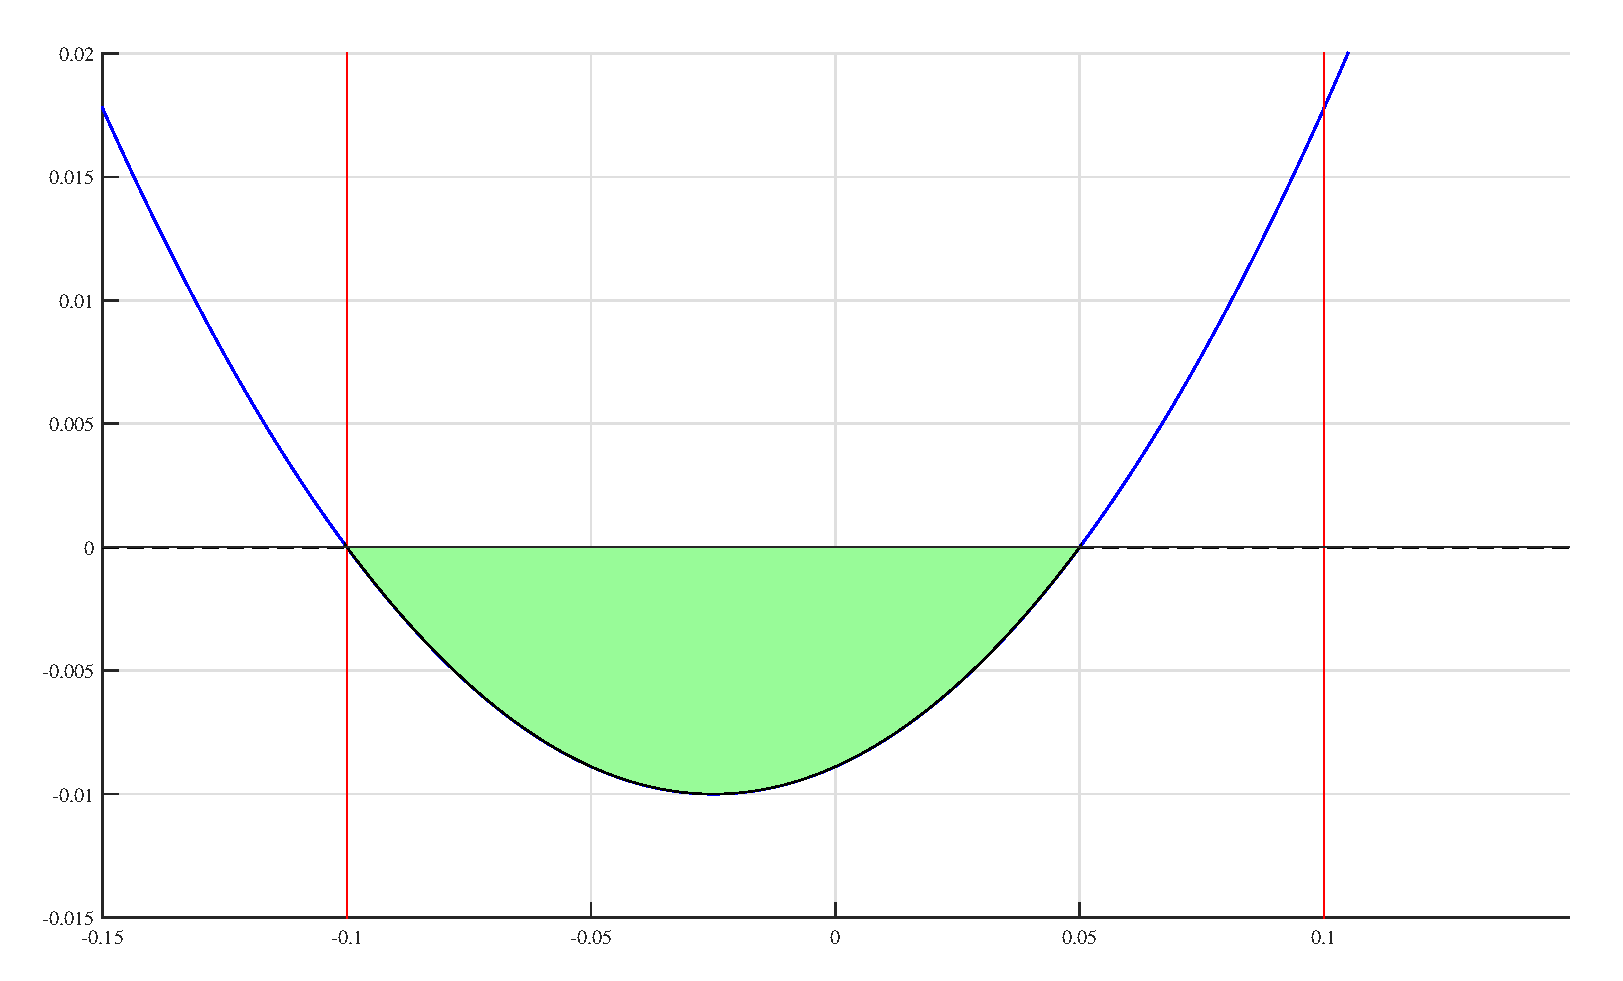
\includegraphics[width=0.4\linewidth]{cbf_1d.eps} \hspace{0.2cm}
			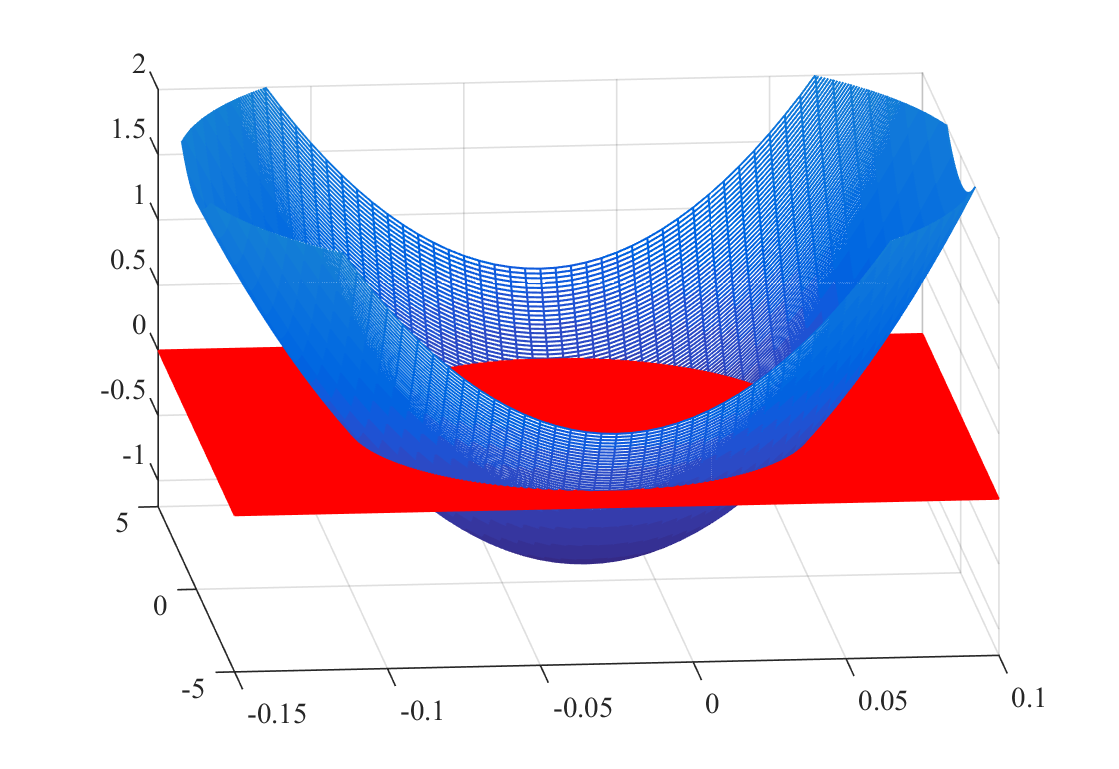
\includegraphics[width=0.4\linewidth]{cbf_2d.eps}
		\item Simulering med Forward Euler
	\end{itemize}
\end{block}
\vspace{-0.7cm}
\scriptsize
\begin{align*}
&\scriptsize \dot{x} = \lambda x \nonumber \\
&\dot{x} = \frac{x_n - x_{n-1}}{t_n - t_{n-1}} = \frac{x_n - x_{n-1}}{h} = \lambda x_{n-1}  \\
& x_n = x_{n-1}(1+h\lambda) = x_0(1+h\lambda)^n \\
&\Rightarrow \,\,\, |1+h\lambda| > 1 \,\,\,\text{ustabil} 
\end{align*}
\end{minipage}
\hspace{0.3cm}
\begin{minipage}{0.35\textwidth}
{\color{white}{white}}\\
{\color{white}{white}}
\hspace*{-0.5cm}
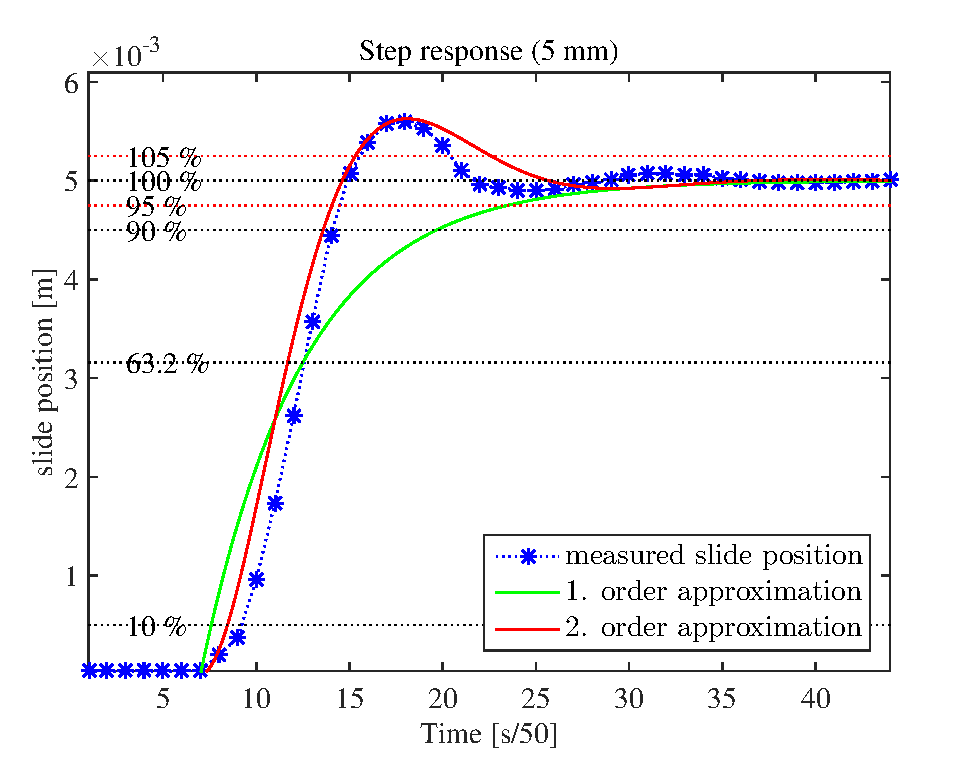
\includegraphics[width=1.1\linewidth]{model_1d.eps}

\hspace*{-0.5cm}
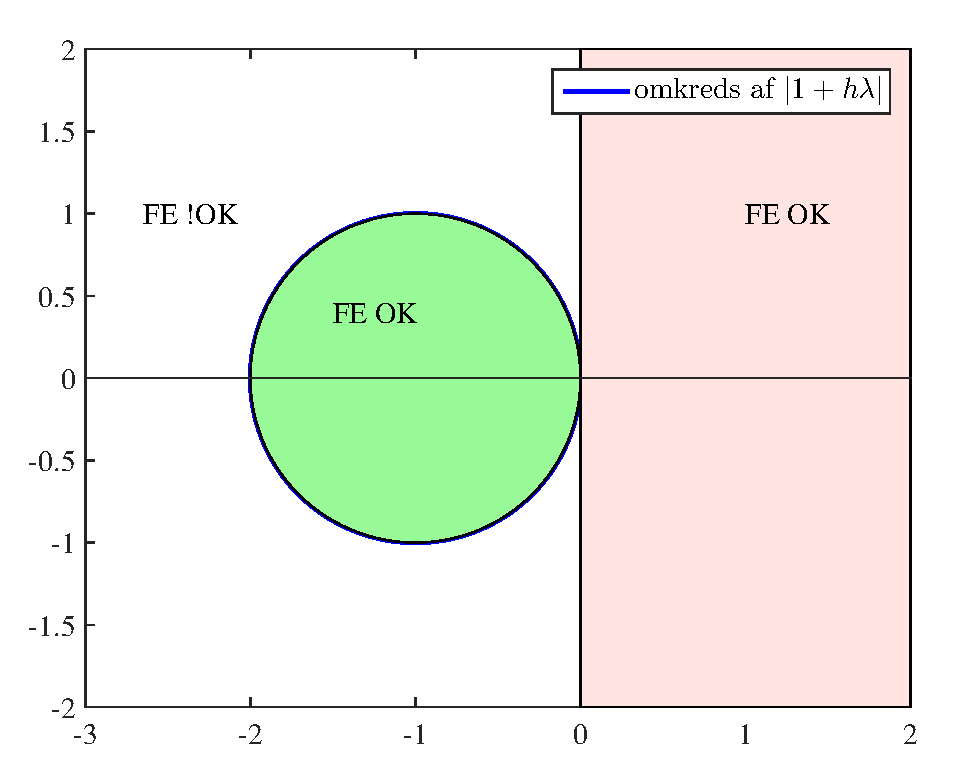
\includegraphics[width=1.1\linewidth]{fe_graphs.eps}

\end{minipage}
\end{frame}


\begin{frame}{Sikkerhed for et 1 dimensionelt system}{Resultater og erfaring}
\begin{minipage}{0.48\textwidth}
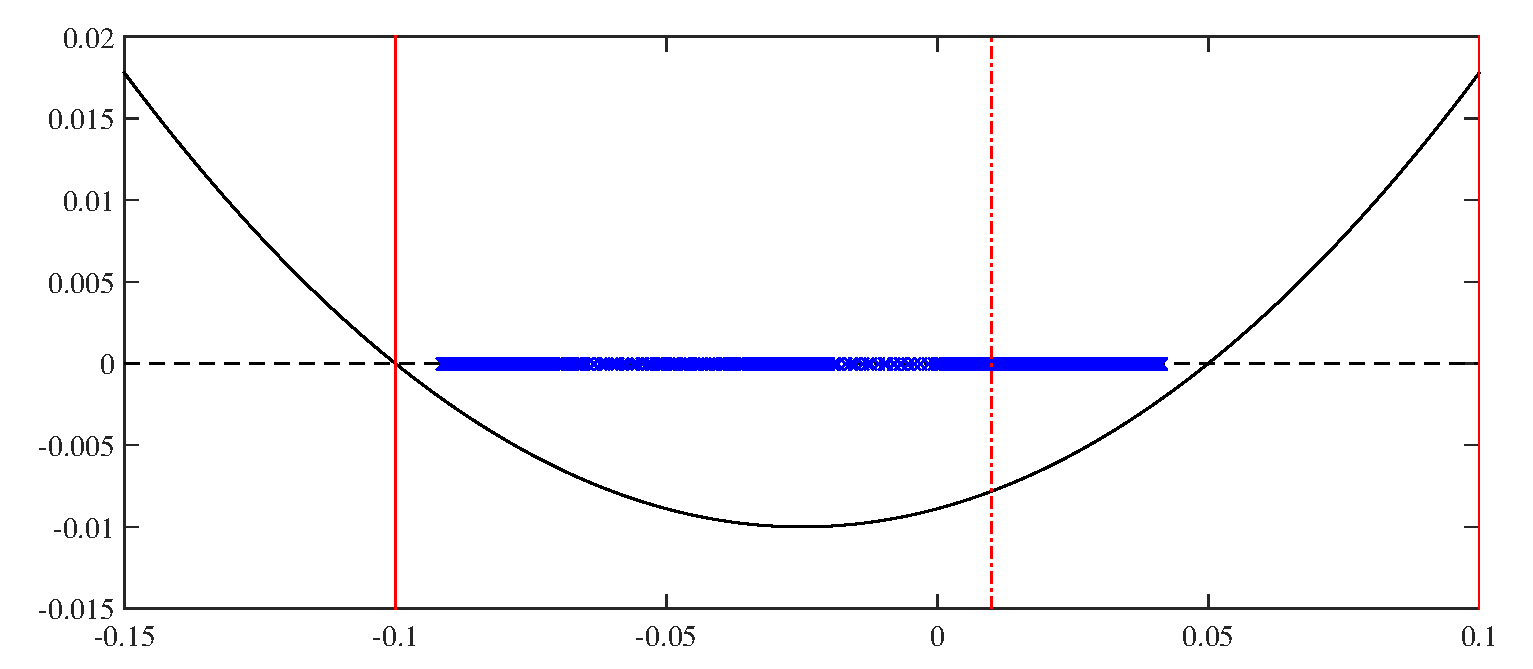
\includegraphics[width=1\linewidth]{plot_states_nem.eps}

\begin{itemize}
%	\item \scriptsize $\tilde{u}(\textbf{x},u) = k_0(\textbf{x})\sigma(\textbf{x}) + ( 1-\sigma(\textbf{x}) ) u(\textbf{x})$
	\item \scriptsize $k_0(\textbf{x}) = -\dfrac{a + \sqrt{a^2 + \kappa^2 b b^T}}{b b^T} b^T$
%	\item \scriptsize $\sigma(\textbf{x}) = \begin{cases} 1 \\ \text{bump function} \\ 0 \end{cases}$
%	\item Betydning af $\kappa$, $\sigma$, ..
%	\item simulering + da Vinci implementering
\end{itemize}


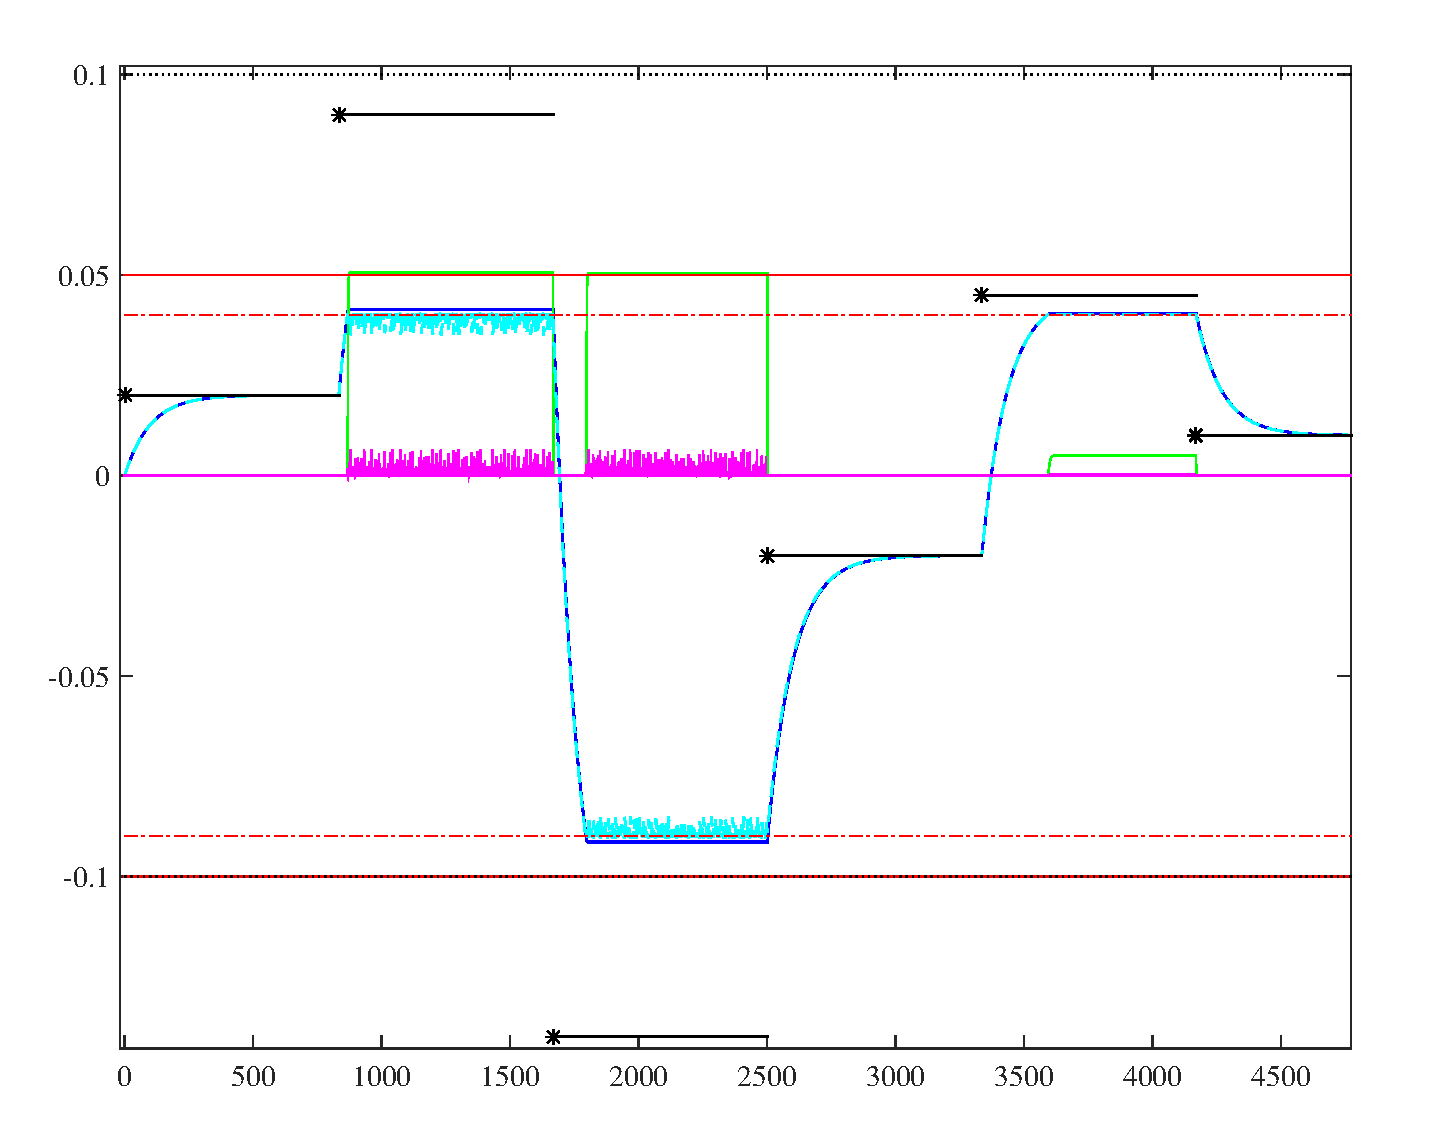
\includegraphics[width=1\linewidth]{vary_kappa.eps}
\vspace*{-0.4cm}


\end{minipage}
\begin{minipage}{0.48\textwidth}
{\color{white}{white}}
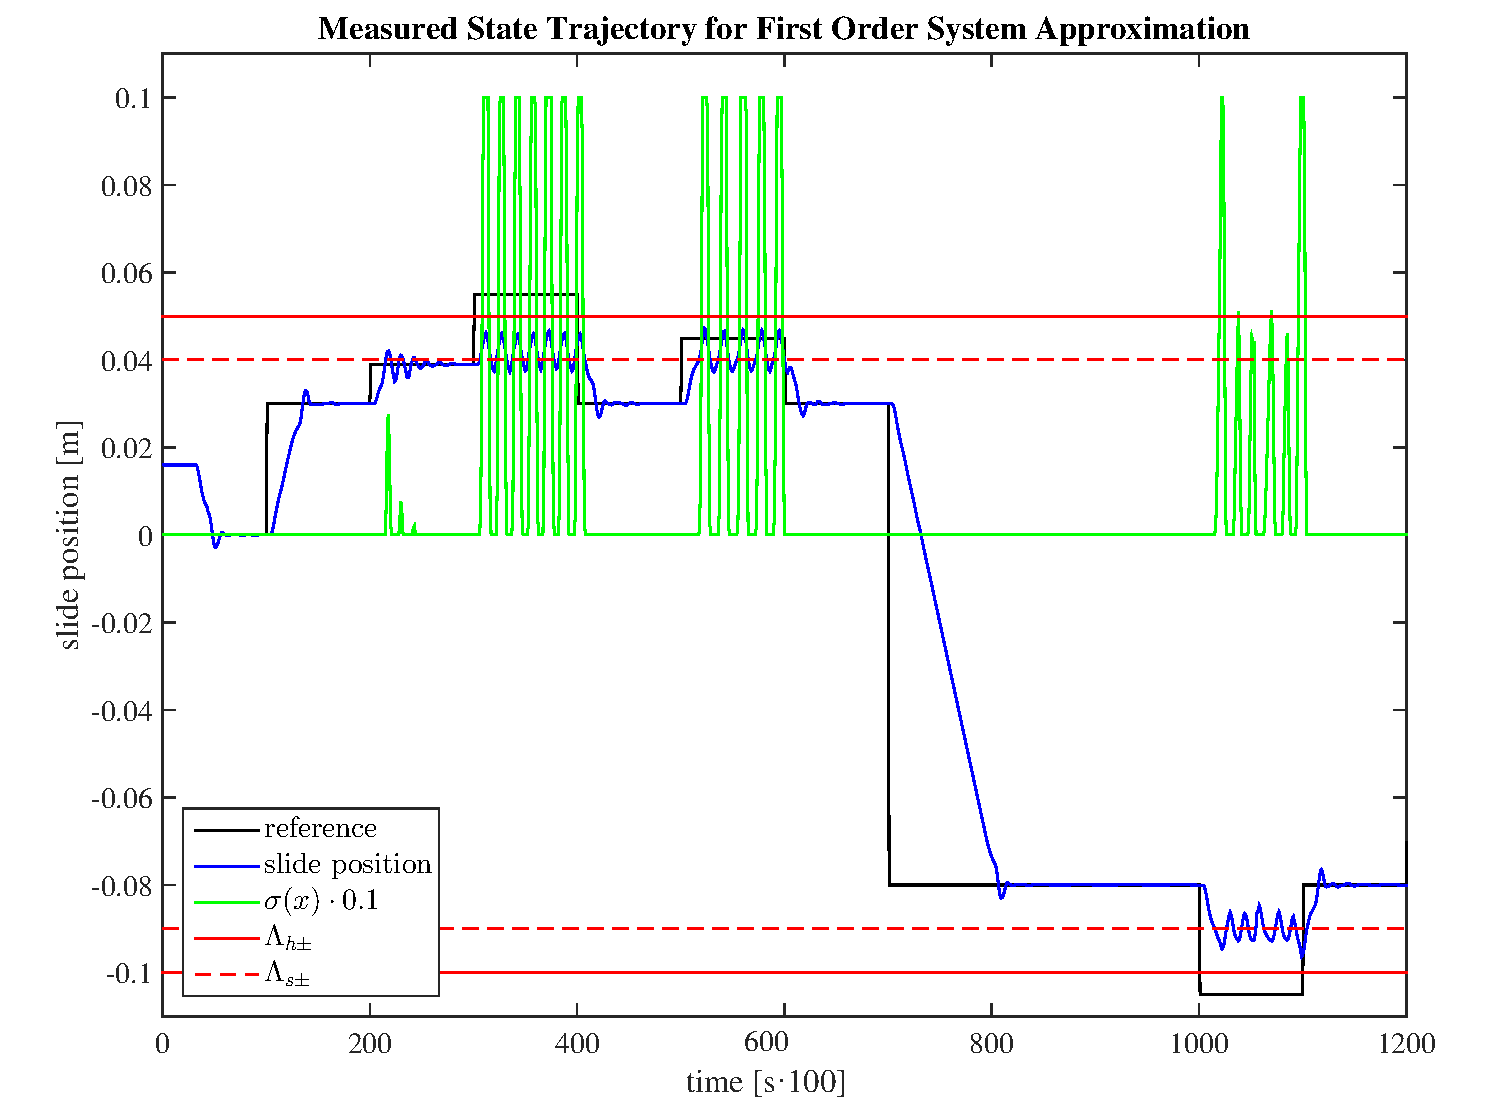
\includegraphics[width=1\linewidth]{trajectory_slide_meas_1-eps-converted-to.pdf}

\vspace*{0.05cm}
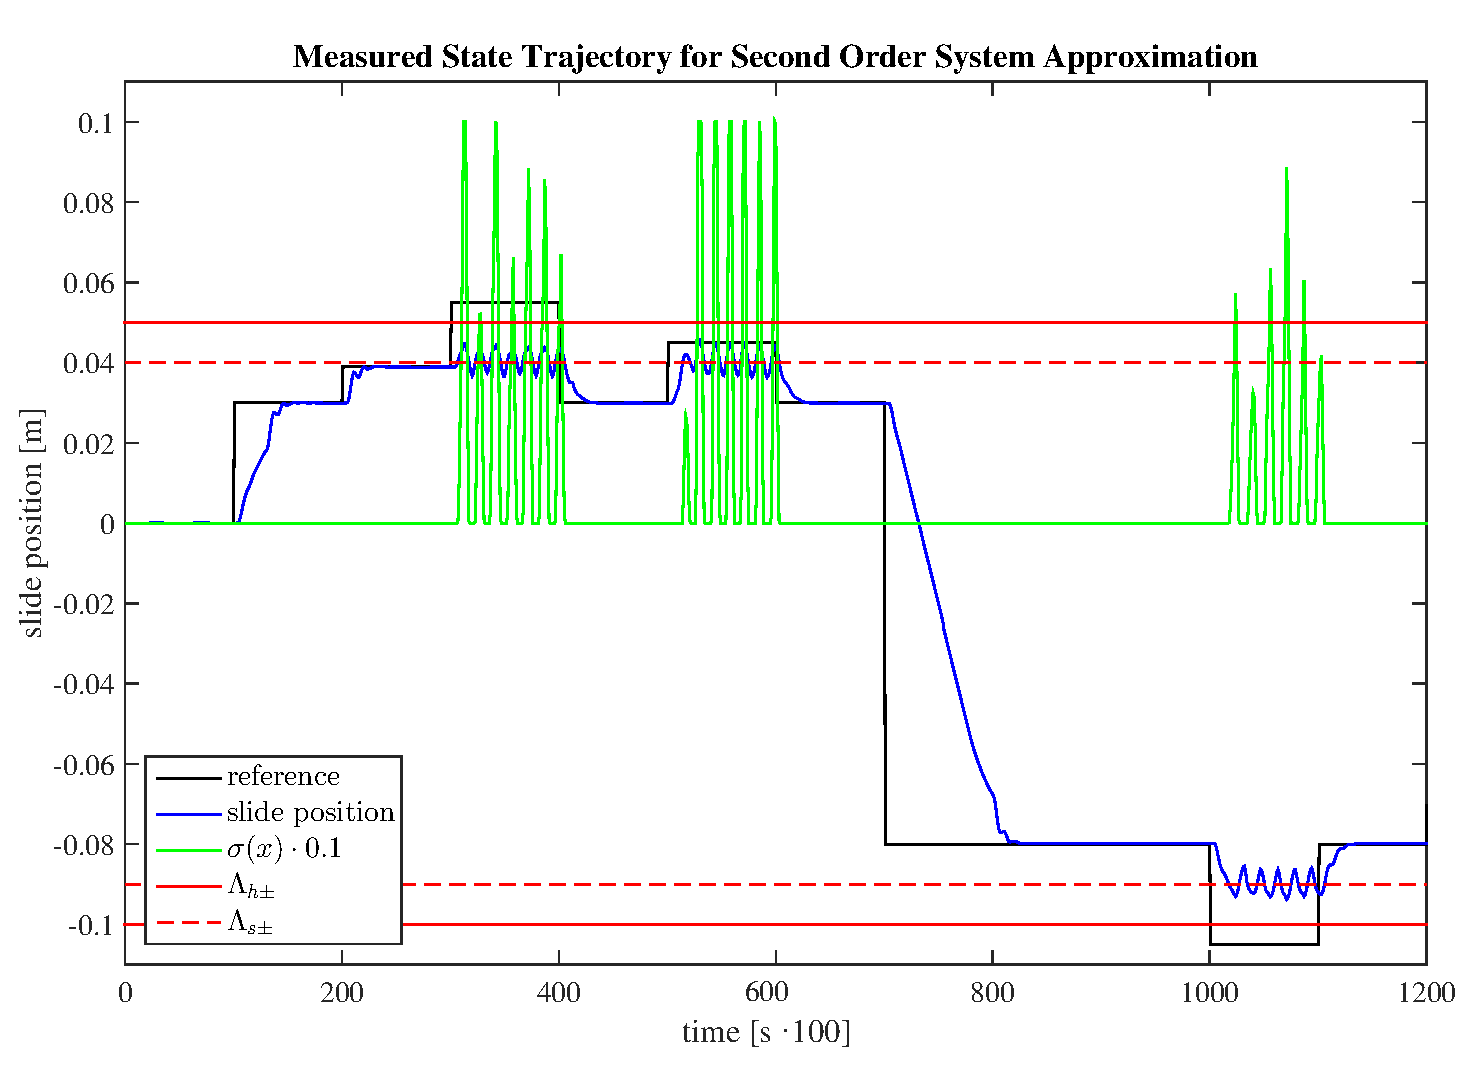
\includegraphics[width=1\linewidth]{meas_trajectory_2_order-eps-converted-to.pdf}

\end{minipage}
\end{frame}

\begin{frame}{Sikkerhed for et dynamisk system}{Indledende udvikling til at opnå virtual fixture}
\section{Virtuel fixture}
\vspace*{-0.7cm}
\begin{block}{}
	\begin{itemize}
		\item Opnå en sikker afstand
		\item Lægen skal opleve hjertet som stillestående
		\item Modeller hjertet som en sinus bevægelse (Dr. Poulsen)
	\end{itemize}
\end{block}
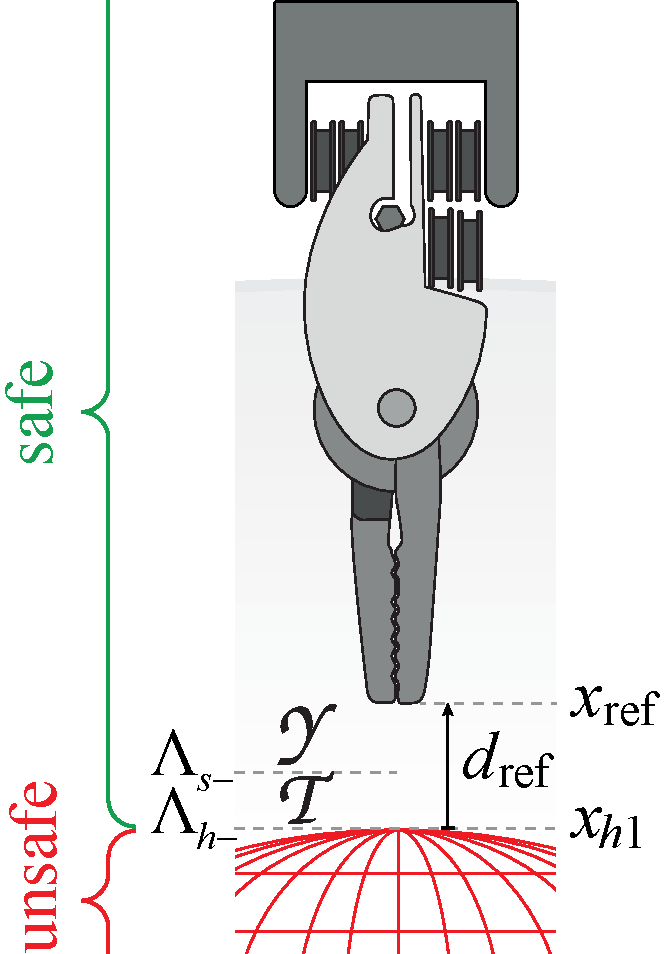
\includegraphics[width=0.175\linewidth]{dynamic_boundary_limits.pdf} \hspace*{0.4cm}
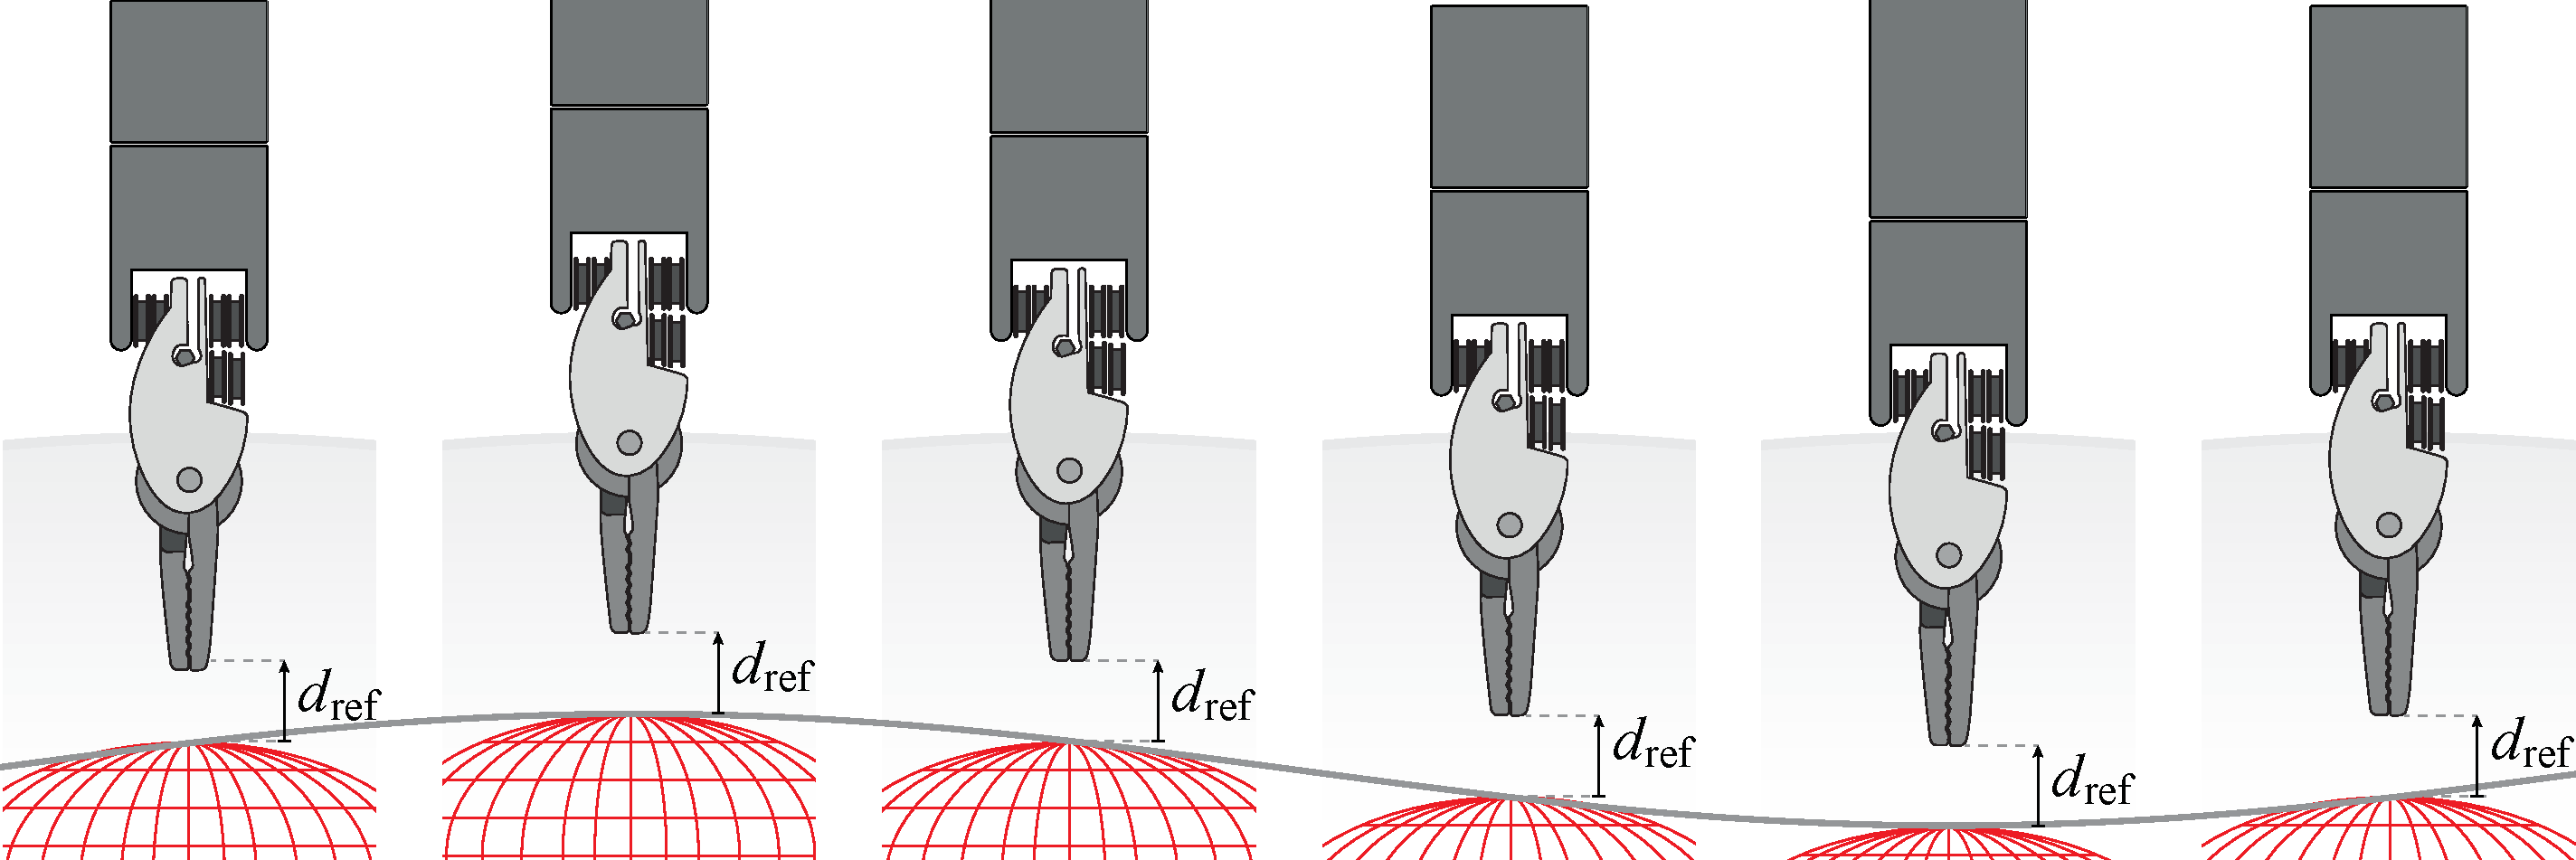
\includegraphics[width=0.75\linewidth]{dynamic_boundary_sequence.pdf}

\begin{minipage}{0.7\textwidth}
\scriptsize
\begin{align*}
& \dot{\textbf{x}} = \begin{bmatrix}
-1/\tau & 0 & 0 & 0 \\
0 & 0 & \omega_h & 0 \\
0 & -\omega_h & 0 & 0 \\
0 & 0 & 0 & 0
\end{bmatrix} \begin{bmatrix}
x_1 \\ x_{h1} \\ x_{h2} \\ d_\text{ref}
\end{bmatrix} + \begin{bmatrix}
1/\tau \\ 0 \\ 0 \\ 0
\end{bmatrix} u \\
&  u = \bar{N} x_\text{ref} - \textbf{K} x_1 = \bar{N}\Big( x_{h1} - x_1 \Big) - \textbf{K} x_1 = \bar{\textbf{K}}x
\end{align*}
\end{minipage}
\hspace*{0.1cm}
\begin{minipage}{0.25\textwidth}
\vspace*{0.2cm}

\includegraphics[width=0.75\linewidth]{barrier.jpg}
\hspace*{-0.3cm}
\vspace*{-0.2cm} \scriptsize
\begin{align*}
B(x) = \tilde{c}\Big( x_{h1} - x_1 \Big){\color{white}{lol}}
\end{align*}
\end{minipage}
\end{frame}

\begin{frame}{Sikkerhed for et dynamisk system}{Resultater}
\hspace*{-0.5cm}
\begin{minipage}{0.46\textwidth}
	\begin{itemize}
		\item Simulering
	\end{itemize}
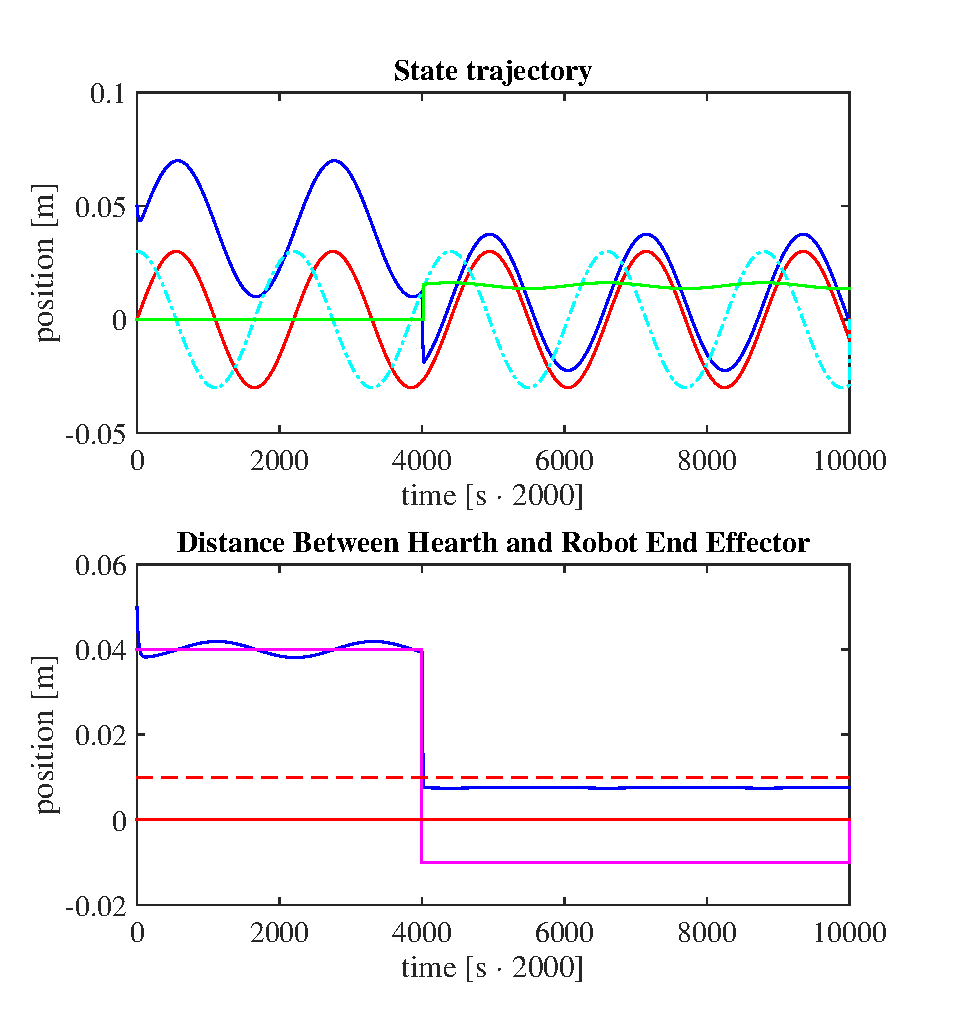
\includegraphics[width=1.17\linewidth]{dyn.eps}
\end{minipage}
\hspace{0.4cm}
\begin{minipage}{0.46\textwidth}
	\begin{itemize}
		\item Implementering
	\end{itemize}
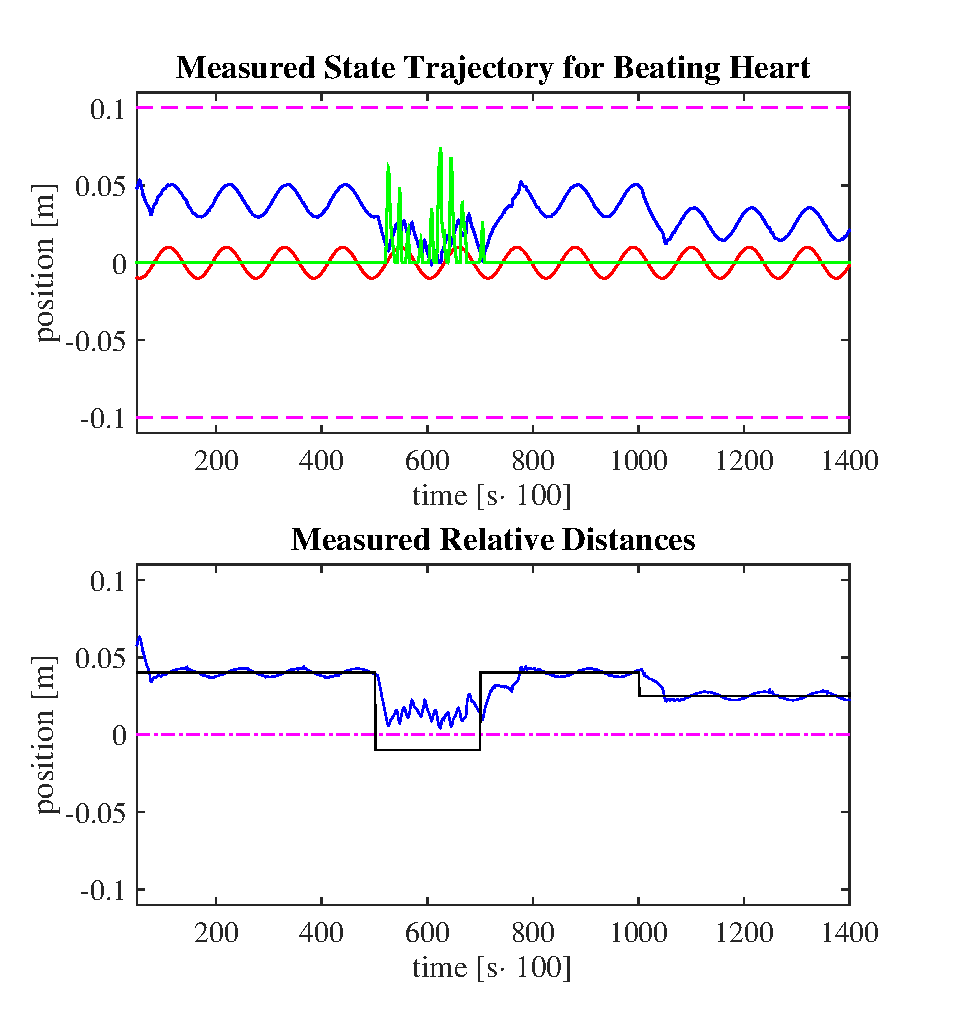
\includegraphics[width=1.17\linewidth]{dyn_meas.eps}
\end{minipage}

\end{frame}

\begin{frame}{Sikkerhed i det 3 dimensionelle rum}{På vej mod noget brugbart}
\section{Sikkerhed i 3D}
\begin{itemize}
	\item Linear model hvor \textit{x, y} og \textit{z} er uafhænginge
	\item Kontrol topologi er identisk med 1D systemet
	\item Kortlægge og modifisere den kinematiske kæde
	\item Anvende kinematiske solvere (KDL)
	\item Definere CBF i 3D
\end{itemize}
\begin{minipage}{0.45\textwidth}
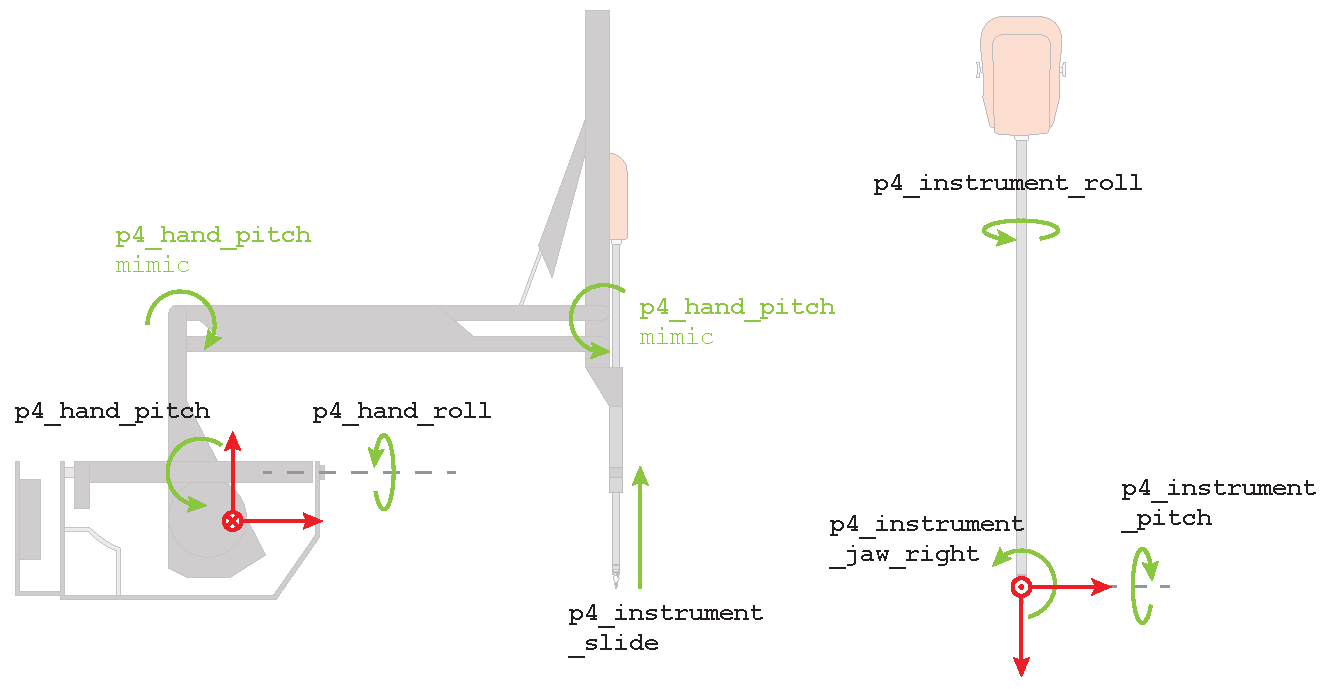
\includegraphics[width=1.2\linewidth]{simple_kinematics.pdf}
\end{minipage}
\hspace*{0.8cm}
\begin{minipage}{0.45\textwidth}
\includegraphics[width=1\linewidth]{3d_bar_ny.eps}
\end{minipage}
\end{frame}

\begin{frame}{Sikkerhed i det 3 dimensionelle rum}{Resultater}
\hspace*{-0.2cm}
\begin{minipage}{0.46\textwidth}
\begin{itemize}
	\item Simulering
\end{itemize}
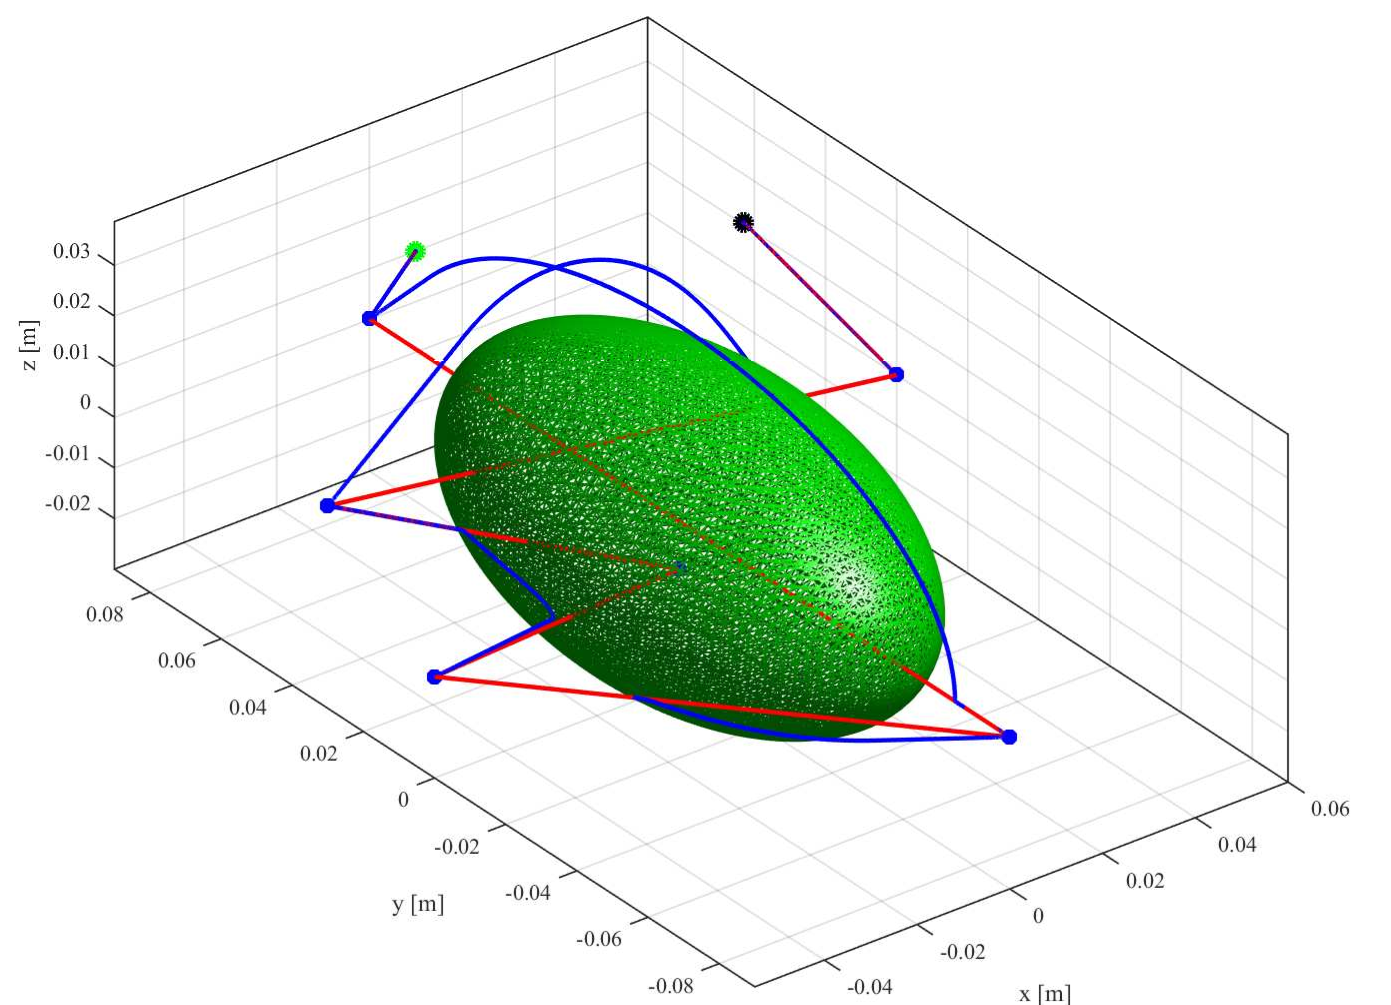
\includegraphics[width=1.0\linewidth]{traj_3d_1_sim.pdf}
\begin{itemize}
	\item Finder setpoints i $\mathcal{X}_0$
	\item Undgår $\mathcal{X}_u$ selvom setpoint er sikker
	\item Finder steady state i nærmeste sikre område
\end{itemize}
\end{minipage}
\hspace{0.2cm}
\begin{minipage}{0.46\textwidth}
\begin{itemize}
	\item Implementering
\end{itemize}
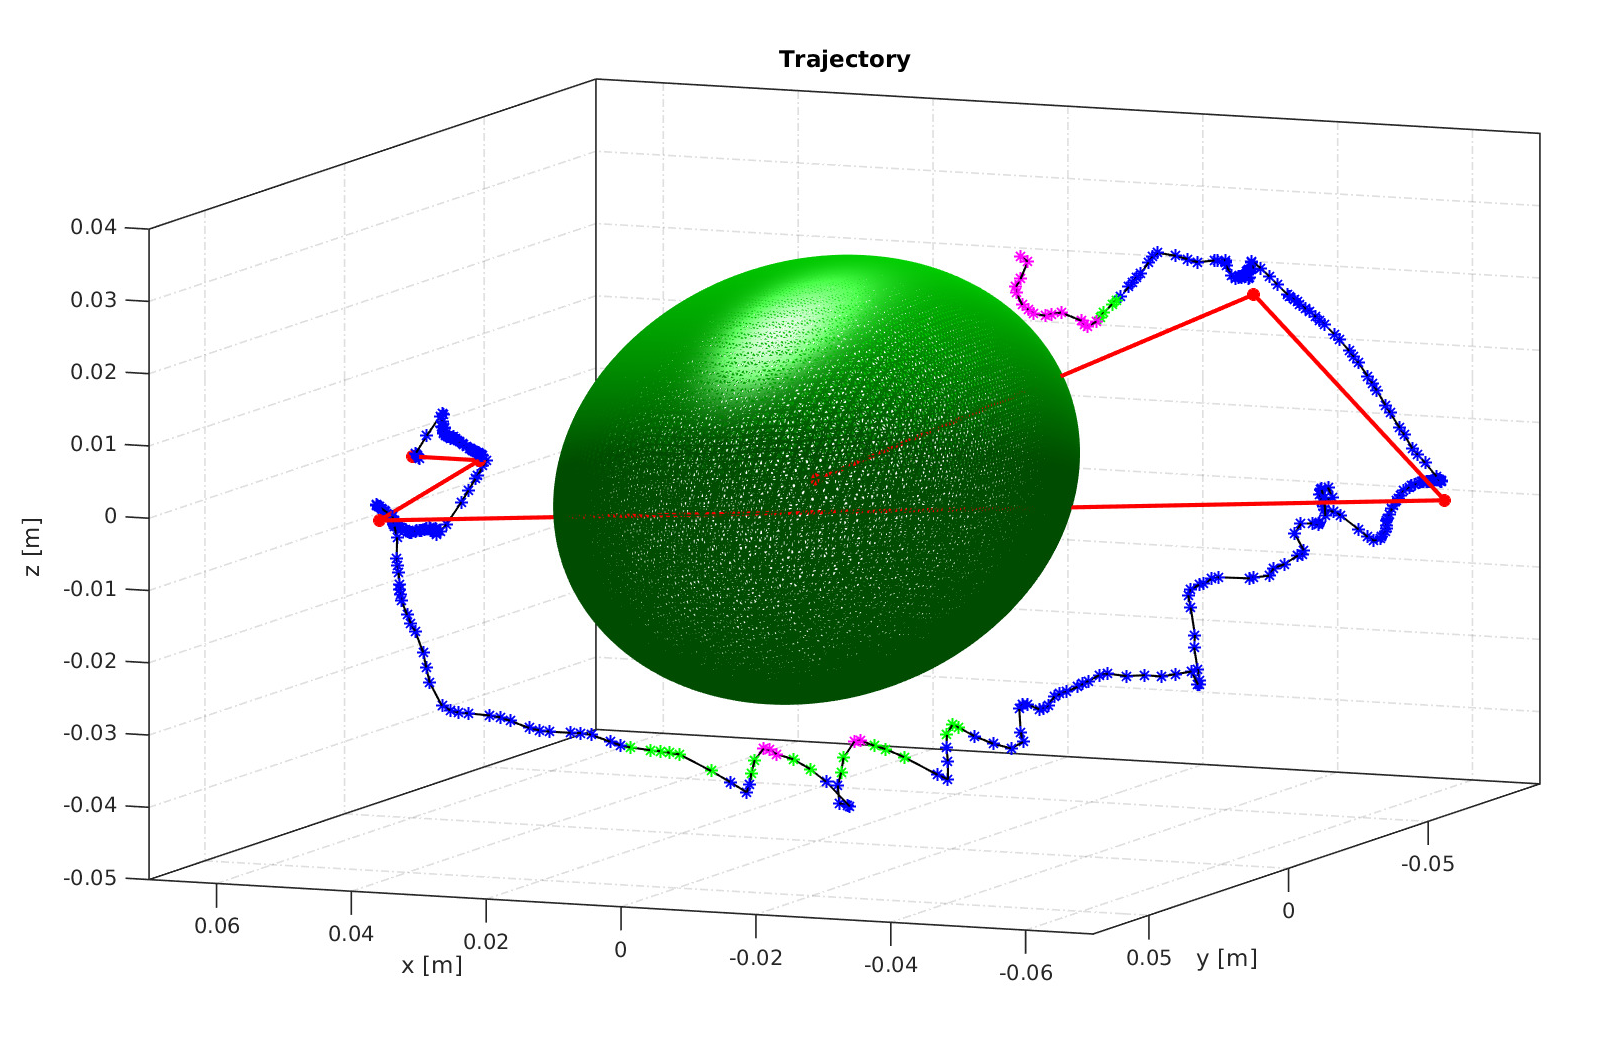
\includegraphics[width=1.1\linewidth]{traj_3d_meas-eps-converted-to.pdf}
\begin{itemize}
	\item Samme karakteristik som simulering
	\item En smule upræcis
	\item IK-solver finder ulogisk løsning - dog en løsning
\end{itemize}
\end{minipage}
\end{frame}

\section{Sikkerhedsverifikation}
\begin{frame}{Sikkerhedsverifikation}{Omformulering af definition for barrierecertifikat}
	\vspace{3mm}
\begin{block}{SOSTOOLS}
	\begin{itemize}
		\item Metodisk måde at søge barrierecertifikat for et system og dermed sikkerhedsvalidere det
		\item Kræver omformulering til sum of squares (SOS) problem
	\end{itemize}
\begin{equation*}
p(\mathbf{x})=\sum\limits_{j=1}^{m}f_j^2(\mathbf{x})=\mathbf{z}^T\mathbf{Q}\mathbf{z}\quad \in\Sigma[\mathbf{x}]
\end{equation*}
\end{block}
	\vspace{-8mm}
\begin{minipage}[b]{0.57\linewidth}
	\phantom{.}
	\vspace*{6mm}
\begin{block}{Putinars Positivstellensatz}
	\begin{itemize}
		\item Gør det muligt at definere funktionens fortegn på de forskellige regioner
	\end{itemize}
	\vspace{5mm}
\end{block}
\end{minipage}
\hspace{1mm}
\begin{minipage}[b]{0.35\linewidth}
	\vspace{3mm}
	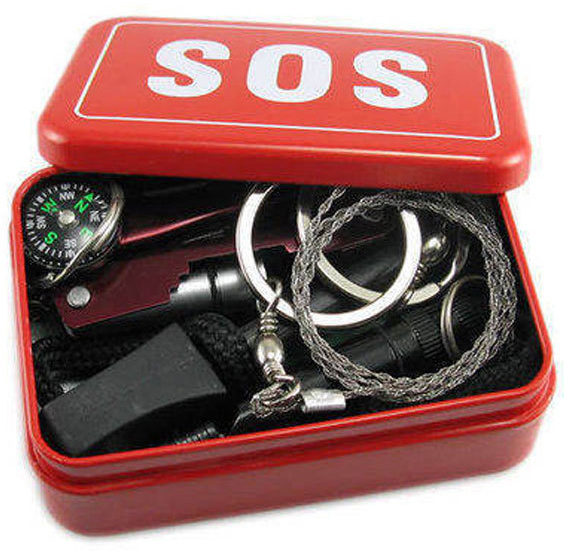
\includegraphics[width=1\textwidth]{sostools.jpg}
\end{minipage}
\end{frame}

\begin{frame}{Barrierecertifikat-søgning med SOSTOOLS}{Sikkerhedsverifikation af lukketsløjfesystem}
	\vspace{2mm}
\begin{minipage}[b]{0.35\linewidth}
	\begin{block}{Barrierecertifikat}
		\vspace{-5mm}
		\begin{align*}
		B(\mathbf{x})&\leq 0 \quad \forall\,\,\,\mathbf{x}\in\mathcal{X}_0\\
		B(\mathbf{x})&> 0 \quad \forall\,\,\,\mathbf{x}\in\mathcal{X}_u\\
		L_{f_{cl}}B(\mathbf{x})&\leq 0 \quad \forall\,\,\,\mathbf{x}\in\mathcal{X}
		\end{align*}
	\end{block}
\end{minipage}
\hspace{15mm}
\begin{minipage}[b]{0.4\linewidth}
%\begin{block}{Slide: beskrevet ved fejltilstand}
%	\begin{itemize}
%		\item 1.ordens-approksimering
%		\item 2.ordens-approksimering
%	\end{itemize}
%\end{block}
%\begin{figure}[h]
%\begin{subfigure}[h]{.3\textwidth}
%	\centering
%	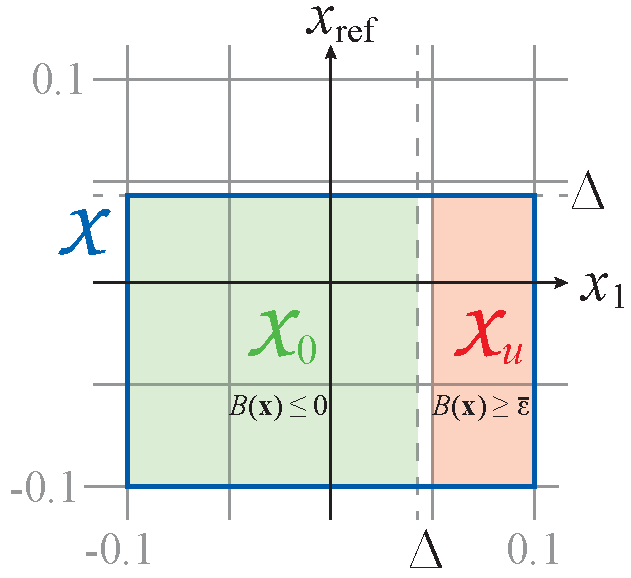
\includegraphics[width=0.3\textwidth]{sos_Xregion.pdf}
%\end{subfigure}
\hspace{3mm}
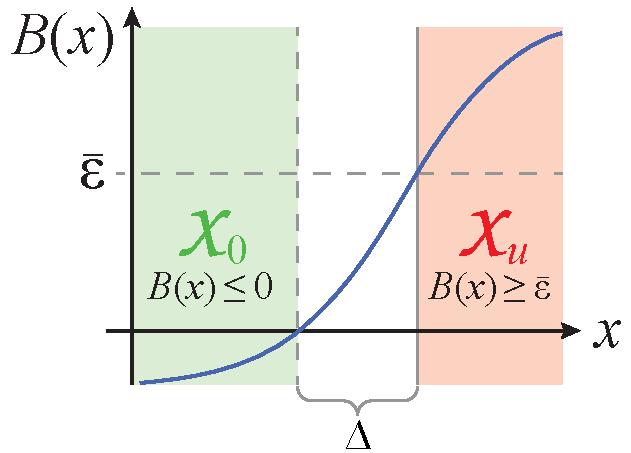
\includegraphics[width=\textwidth]{sos_delta.pdf}
%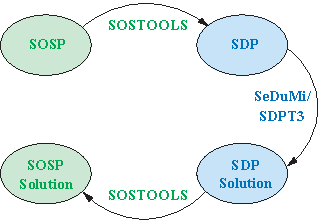
\includegraphics[width=1\textwidth]{SOSTOOLS.pdf}
%\begin{subfigure}[h]{.3\textwidth}
%	\centering
%	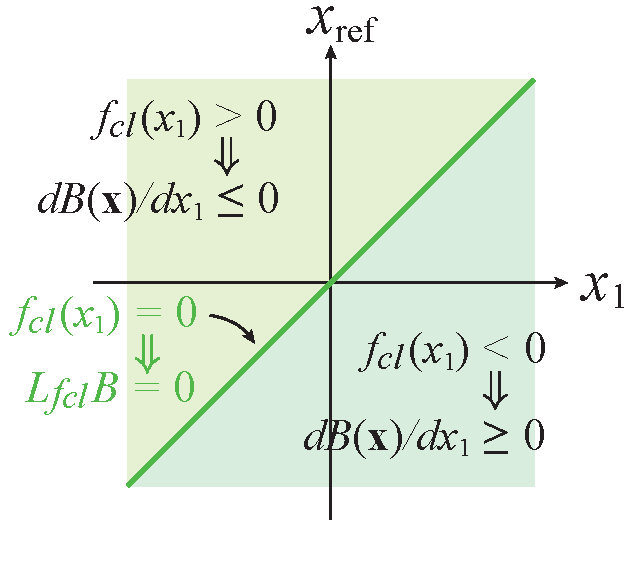
\includegraphics[width=0.4\textwidth]{sos_Xregion_dBdx.pdf}
%\end{subfigure}
%	\hspace{3mm}
%\begin{subfigure}[h]{.3\textwidth}
%	\centering
%	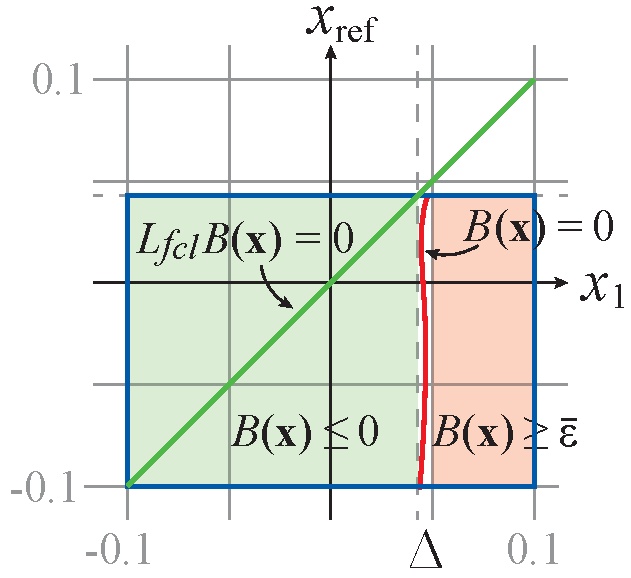
\includegraphics[width=0.3\textwidth]{sos_Xregion_Bvalue.pdf}
%\end{subfigure}
%\end{figure}
%\hspace{3mm}
%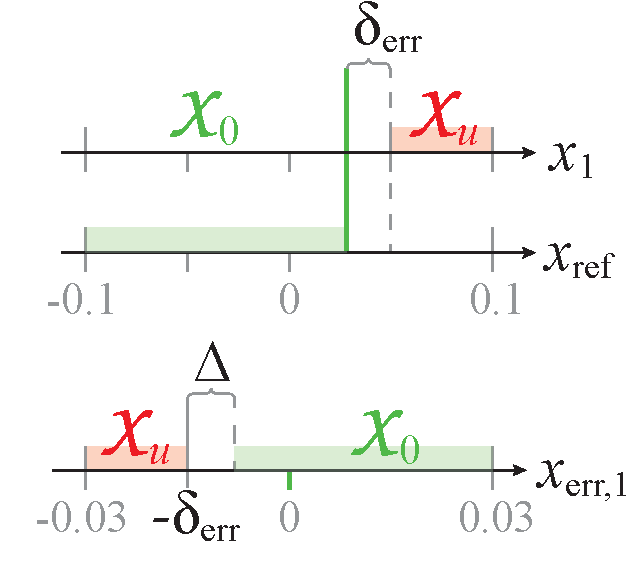
\includegraphics[width=0.4\textwidth]{sos_errorref_1d_new_2ndorder.pdf}
\end{minipage}

%\begin{minipage}[b]{0.65\linewidth}
\vspace{2mm}
%\begin{block}{Forståelse af værktøjet}
%		\begin{itemize}
%			\item Parametre til evaluering af resultat: feasibility ratio, residual norm, test om udtryk er SOS
%		\end{itemize}
%\end{block}
\begin{block}{Omformulering af barrierecertifikat}
	\vspace{-5mm}
	\begin{align*}
	&&	-B(\mathbf{x}) &\geq 0 \quad  \forall \hspace{2mm} \mathbf{x} \in \mathcal{X}_0 \quad \Leftarrow& 	-B(\mathbf{x}) - \sum q_jg_j &\,\,\,\in \Sigma[\mathbf{x}] &&& \\
	&&	B(\mathbf{x})-\bar{\epsilon} &\geq 0 \quad  \forall \hspace{2mm} \mathbf{x} \in \mathcal{X}_u \quad \Leftarrow& 	B(\mathbf{x})-\bar{\epsilon} - \sum q_jg_j &\,\,\,\in \Sigma[\mathbf{x}] &&& \\
	&&	-L_{f_{cl}}B(\mathbf{x}) &\geq 0 \quad  \forall \hspace{2mm} \mathbf{x} \in \mathcal{X} \quad\,\, \Leftarrow& 	-L_{f_{cl}}B(\mathbf{x}) - \sum q_jg_j &\,\,\,\in \Sigma[\mathbf{x}] &&& 
	\end{align*}
\end{block}
%\hspace{1mm}
%\begin{minipage}[b]{0.32\linewidth}
%\href{file:../../MATLAB/test_barriersearch.m}{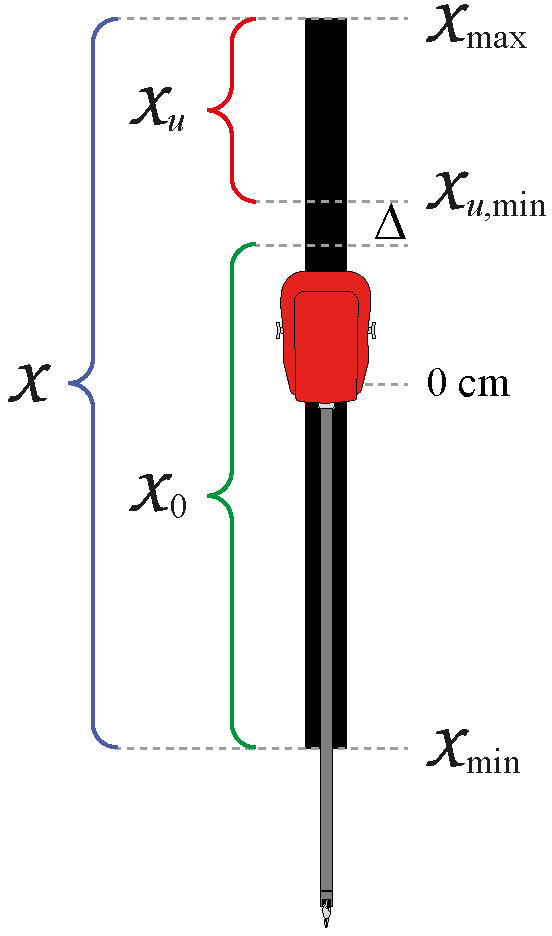
\includegraphics[width=1\textwidth]{slide_sos.pdf}}	
%\end{minipage}
\end{frame}

%\begin{frame}{Barrierecertifikat-søgning med SOSTOOLS}{Sikkerhedsverifikation gennem fejl-tilstand}
%	\begin{block}{Omformulering af problemet til fejl-tilstanden}
%		\begin{itemize}
%			\item Koordinatskifte og sammenhæng
%			\item Forsimpling af problemet -- sikkerhedsverificering af både første- og andenordens model af slide-bevægelse
%		\end{itemize}
%	\end{block}
%	\begin{figure}[h]
%%		\begin{subfigure}[h]{.3\textwidth}
%%			\centering
%			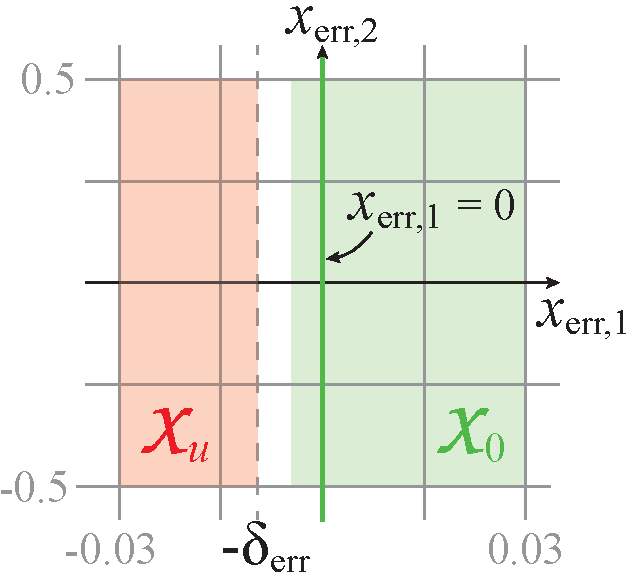
\includegraphics[width=0.3\textwidth]{sos_error_2d_2ndorder.pdf}
%%		\end{subfigure}
%		\hspace{3mm}
%%		\begin{subfigure}[h]{.3\textwidth}
%%			\centering
%			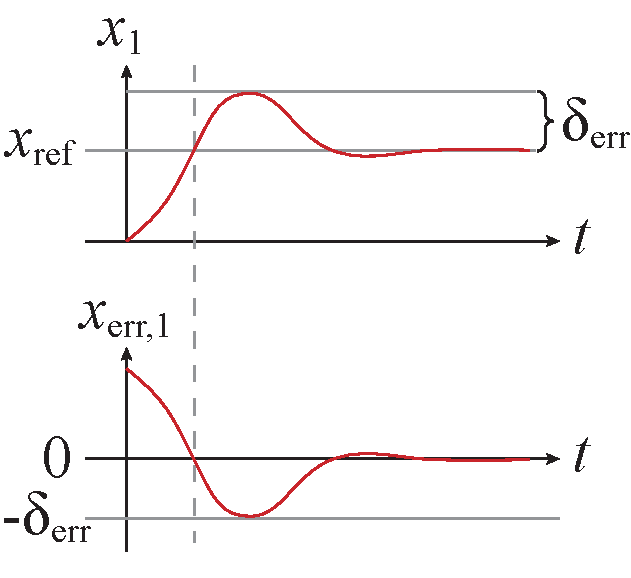
\includegraphics[width=0.3\textwidth]{sos_delta_error_2ndorder.pdf}
%%		\end{subfigure}
%		\hspace{3mm}
%%		\begin{subfigure}[h]{.3\textwidth}
%%			\centering
%			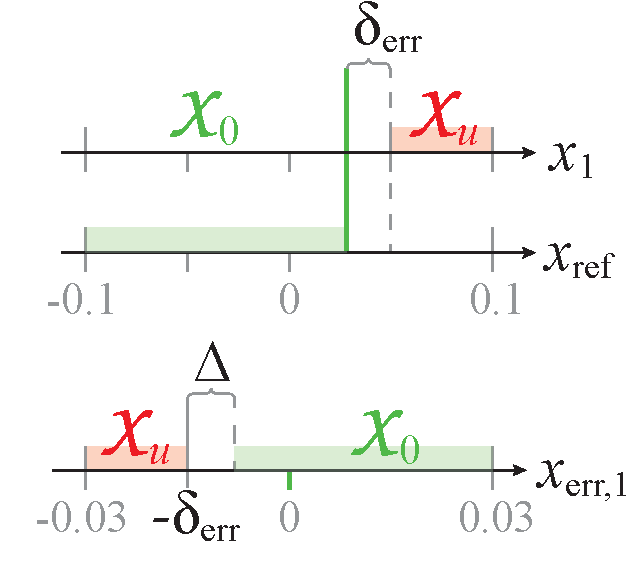
\includegraphics[width=0.3\textwidth]{sos_errorref_1d_new_2ndorder.pdf}
%%		\end{subfigure}
%	\end{figure}
%\end{frame}

%\begin{frame}{Evaluering af SOSTOOLS}{Sikkerhedsverifikation af lukketsløjfesystem}
%	\begin{block}{Evaluering af løsning}
%		\begin{itemize}
%			\item Feasibility ratio, residual norm, test om ligninger er SOS
%			\item Mange parametre at skrue på
%			\item Længere proces at minimere numeriske fejl
%		\end{itemize}
%	\end{block}
%	\begin{block}{Evaluering af værktøjet}
%		\begin{itemize}
%			\item Udviklet framework til søgning efter barrierecertifikater
%			\item Fundet mange brugbare løsninger
%			\item Systematisk afsøgning er en lang og iterativ proces
%			\item Avanceret metode der kommer til sin ret for højere-ordens systemer
%		\end{itemize}
%	\end{block}
%\end{frame}
\begin{frame}{Konklusion}{Har vi flyttet noget?}
\section{Konklusion}
\begin{minipage}{0.6\textwidth}
\begin{block}{}
	\begin{itemize}
		\item \textbf{Et narturligt ønske:}\\ - Sikkerhed og virtual fixture
		\item \textbf{Opdelt løsningsstrategi:}\\ - Design og Analyse 
		\vspace{0.3cm}
		\item Sikkerhed \underline{kan} garanteres
		\item virtual fixture \underline{kan} opnås
		\item Success i begge tilgange \\
		\scriptsize - design og analyse
		\item \normalsize Interfacing gennem ROS er klargjort + kortlægning af den kinematiske kæde og IK.
		\item En stejl læringskurve er brudt \\ 
		\scriptsize - der kan arbejdes videre på projektet
	\end{itemize}
\end{block}
\end{minipage}
\begin{minipage}{0.35\textwidth}

\includegraphics[width=1\linewidth]{blowing-a-dandelion-600.jpg}
\vspace*{0.2cm}


\includegraphics[width=1\linewidth]{TwoPaths-900x470.jpg}
\vspace*{0.2cm}


\includegraphics[width=1\linewidth]{path-to-success.jpg}
\end{minipage}
\end{frame}

\begin{frame}{Konklusion}{Konklusion på design tilgangen}
\begin{itemize}
	\item Relativ intuitiv design procedure \\	\vspace*{0.08cm}
	\scriptsize {\color{white}{m}} 1. Lav model \\	
    \scriptsize {\color{white}{m}} 2. Konstruer CBF udfra fysiske forhold og beregn Lie afledede\\	
    \scriptsize {\color{white}{m}} 3. Specificer $\epsilon$ sådan at $\mathcal{T}$ er "tilpas" \\	
    \scriptsize {\color{white}{m}} 4. Design en vilkårlig controller i det sikre område \\ 	
    \scriptsize {\color{white}{m}} 5. Kombiner "sikker" og "usikker" controller \\
	\item \normalsize Kreativitet er nødvendigt når en CBF skal konstrueres
	\item Brug når der er et fysisk forhold til tilstandene
	\item Brugbar og behagelig fremgangsmåde
\end{itemize}
\vspace*{0.2cm}

\includegraphics[width=0.27\linewidth]{checklist.jpg} \hspace*{0.2cm}

\includegraphics[width=0.35\linewidth]{p01tgd39.jpg} \hspace*{0.2cm}
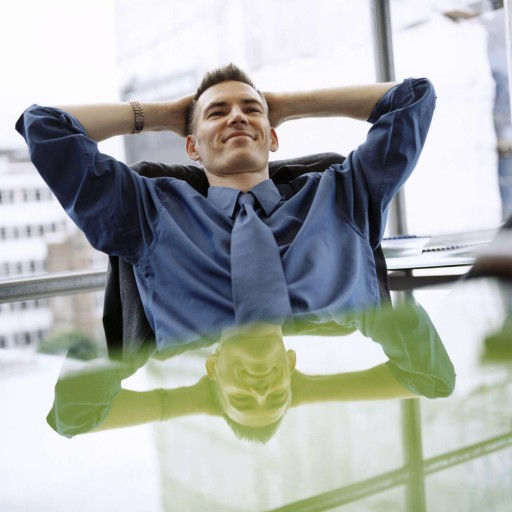
\includegraphics[width=0.2\linewidth]{9212_fit512.jpg}
\end{frame}



\begin{frame}{Konklusion}{konklusion på analyse tilgangen}
\begin{itemize}
	\item Global (SOS) til lokal (putinar positivstellensatz)
	\item Et framework er udviklet
\end{itemize}

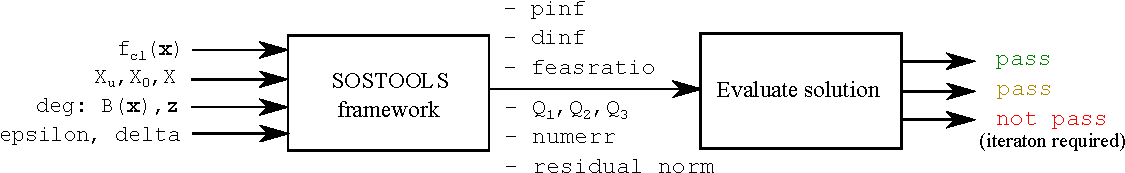
\includegraphics[width=1\linewidth]{sostools_eval.pdf}

\begin{itemize}
%	\item Frameworket kan udvides til \textit{n}-dimensioner
	\item \textbf{Anvendelse:} Forstå betydningen af $\Delta, \epsilon, g_j$ og $deg$.
	\item \textbf{Budskab:} Når en grøn løsning er fundet - Stop
	\item \textbf{Udvidelse i dimensioner:} Trivielt, men der skal defineres nye intervaller for \textit{g} polynomier 
	\item Abstrakt teori er analyseret, anvendt sammen med SOSTOOLS og en guide er udarbejdet
\end{itemize}

\end{frame}

\begin{frame}{Fremtidigt arbejde}{Vi er ikke stærkere end det svageste led i kæden}
\begin{minipage}{0.65\textwidth}
\begin{block}{}
	\begin{itemize}
		%\item Fejl-tolerant kontrol % \\ 
		%\scriptsize {\color{white}{m}} - Hvad hvis vi mister en sensor?
		\item \normalsize Kompleksitet af barrier funktioner
		\item \normalsize Robust/fejl-tolerent kontrol %\\ 
%		\scriptsize {\color{white}{m}} - Modeller vil altid være forsimplet!
		\item \normalsize Inkorporere Integral virkning \\ 
		\scriptsize {\color{white}{m}} - især tydeligt ved det dynamiske system
%		\item lave en tre delining i $\mathcal{T}$
		\item \normalsize End effector orientering \\
		\scriptsize {\color{white}{m}} -  Sikre sikkerhed for rammen
		\item \normalsize  Trajektorie planlægning \\ 
		\scriptsize {\color{white}{m}} - hvis springet mellem \textit{x} og \textit{x}$_{\text{ref}}$ er for stort
		\item \normalsize Tachometer kan blive "forvirret"
		\item Skræddersy IK solver
		\item Øge sampling rate til 2\,kHz \\
		\scriptsize {\color{white}{m}} - UDP i stedet for TCP/IP
		\item \normalsize  Monte Carlo simulering ved brug af SOSTOOLS framework
	\end{itemize}
\end{block}
\end{minipage}
\begin{minipage}{0.3\textwidth}
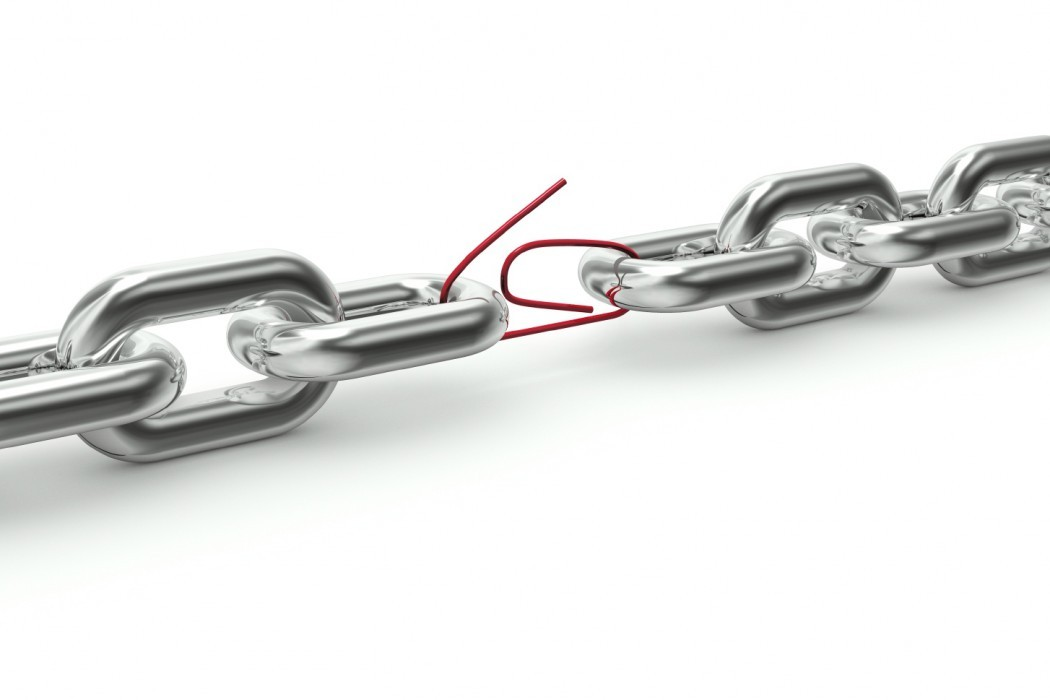
\includegraphics[width=1\linewidth]{The-Weak-Link-in-the-Chain-474557-2.jpg}
\vspace*{0.2cm}


\includegraphics[width=1\linewidth]{work_with_us.jpg}
\vspace*{0.2cm}


\includegraphics[width=1\linewidth]{chain-links-WEB.jpg}
\end{minipage}
\end{frame}

{\aauwavesbg%
\begin{frame}[plain,noframenumbering]%
  \finalpage{Demo}
\end{frame}}
%%%%%%%%%%%%%%%%

\end{document}
